%en:
%Online NIH format requires to separate the \sections. Do this by just
%uncommenting the \clearpage before each \section command. Then can use
%the 'save marked pages' function in gv to split the file and then
%use ps2pdf to make separate pdf files.
%en Add PMCID as a note in bibtex, plainnat shows it. 
%
%Or use pdftk, as in (for page 1):
%pdftk grant.pdf cat 1 output SpecificAims.pdf
%pdftk grant.pdf cat 14-17 output Bibliography.pdf

\documentclass[11pt]{article}
%\documentclass[11pt,notitlepage]{nihblank} %I think this is the old
                                            %format, not needed 

% Packages to load

% Palatino font that NIH allows
\usepackage[T1]{fontenc}
\usepackage[sc]{mathpazo}
\linespread{1.05} %palatino needs a bit more space

% For upright Greek letters in units, such as {\textmu}m
\usepackage{textcomp} 

% For Inkscape figure imports
\usepackage{color}
\usepackage{import}

% Better and richer math environment
\usepackage{amsmath}

% EPS and PDF figures
\usepackage{graphicx}

% Side captions of figures
%\usepackage{sidecap}

% More flexible figure legends
\usepackage[labelfont=bf]{caption}
%\usepackage[labelfont=bf,hang]{caption}

% Nicer tabular environment
\usepackage{booktabs}

% Make 0.5'' margins on all sides
\usepackage[top=0.5in,bottom=0.5in,left=0.5in,right=0.5in]{geometry}

% No page numbers
\pagestyle{empty}

% Hyphenation hints
\hyphenation{ionto-pho-re-tic iso-tro-pic}

%en Following added my me  --Ernst Niebur, March 2012 (originally February 2008)
%\usepackage{subsections} %this, and the same-named option in the first
			 %line, allow to use deeper subsections
\long\def\comment#1{} %%% to comment out a section of text
\usepackage{wrapfig}     %wrap text around figs
%\usepackage{/home/niebur/biblio/bibtex/theapa}
\usepackage[authoryear]{natbib} %first citation is full authorlist
%\usepackage[longnamesfirst]{natbib} %first citation is full authorlist
%\usepackage[numbers,sort&compress]{natbib} %use numbers to save space
\usepackage[small,compact]{titlesec}  %save space
\usepackage{xspace}  
%Change how sections are labelled. We use  A.1.a etc. 
\renewcommand\thesection{\Alph{section}}
\renewcommand\thesubsection{\thesection.\arabic{subsection}}
\renewcommand\thesubsubsection{\thesubsection.\alph{subsubsection}}
\newcommand{\ie}[0]{{\em i.e.}\xspace}
\newcommand{\eg}[0]{{\em e.g.}\xspace}
\newcommand{\etal}[0]{{\em et al.}\xspace}
\newcommand{\etc}[0]{{\em etc.}\xspace}
\newcommand{\vs}[0]{{\em vs.}\xspace}
\newcommand{\vv}[0]{{\em vice-versa}\xspace}
\comment{
If you use the AucTeX-mode with your Emacs, you can switch the output
type between pdf and dvi by typing C-c C-t C-p. Then AucTeX uses
pdflatex which handles png-files by default.

To have pdf output enabled by default with AucTeX, you can put
something like this in our .emacs: (setq TeX-PDF-mode t) 

To enable it just for the one particular file each time it is loaded,
add something like this to the end of your file:
%%% Local Variables:
%%% mode: latex
%%% TeX-PDF-mode: t
%%% End:
}

%en End of my additions  --Ernst Niebur

% bh (added for formatting purposes)

% Indent after section headings
%\usepackage{indentfirst}

% bh added for making bold brackets to highlight revisions
\usepackage{bm}

\begin{document}

\ \vspace{20mm}\\

{\LARGE Grouping mechanisms for object-based vision and attention}

\ \\
{\bf \large Brian Hu$^{\displaystyle 1, \displaystyle 2}$}\\
{$^{\displaystyle 1}$Zanvyl Krieger Mind/Brain Institute, Johns Hopkins University, Baltimore, MD}\\
{$^{\displaystyle 2}$Department of Biomedical Engineering, Johns Hopkins University, Baltimore, MD}\\

\ \vspace{20mm}\\

{\bf Committee Members:} Ernst Niebur (advisor), R\"udiger von der Heydt, Kechen Zhang\\

\ \vspace{20mm}\\

{\bf Public Health Significance:} We are interested in how different cortical areas and types of cortical connections contribute to our perception of objects and our ability to attend to objects. Our findings will describe healthy brain function in adults with normal vision, but may also guide treatments or rehabilitation in the diseased brain, such as for cases of object-based neglect.\\

\ \vspace{20mm}\\

{\bf Proposed Research:} This work will investigate whether feedback     grouping mechanisms are fundamental for linking early feature representations to perceptual objects.The proposed modeling experiments will address how visual features are grouped into 2D and 3D object representations.\\

\clearpage

\thispagestyle{empty}

\sloppy %better white space than overruns...

%\section*{Introduction to Resubmission Application}
%We thank the reviewers for their time in critiquing this
%proposal and for providing very helpful suggestions. We
%have made several major changes to address their concerns.
%% $\bm{\{}$\textbf{\textit{Changes are indicated by brackets
%%    and font change
%%%
%%wherever % or whenever? %en both seem ok to me
%%possible.}}$\bm{\}}$ 
%%%
%The sections "Project Summary," "Research Strategy," "Sponsor and Co-sponsor Information," and
%"Specific Aims" have been extensively modified.
%%are too extensive to be marked individually.
%% $\bm{\{}$\textbf{\textit{Minor changes are indicated by brackets
%%    and font change
%%%
%%wherever % or whenever? %en both seem ok to me
%%possible.}}$\bm{\}}$ 
%%not
%%all changes are marked. 
%%en in retrospect, I think you should just say that the changes are
%%too extensive to be marked individually, which is surely true. If
%%not, there is the danger 
%%that reviewers may think that only the marked places are changed and
%%consider that too little modification.
%%
%We have removed analyses related to
%determining the relative contributions of feedforward, feedback, and
%lateral connections in our models
%%en how about this, it seems shorter and simpler:
%to streamline the proposal. 
%% % % % %
%% bh Let me know if this reason is good enough...
%%These analyses potentially confounded model validation and prediction in our original proposal.
%% % % % %
%In their place, we plan to extend our contour grouping model to
%perform segmentation of natural images, a task which is largely
%unstudied from a neurally-realistic modeling perspective. We will also
%provide a more comprehensive theoretical framework for understanding
%how different surfaces can be represented in the brain using basis
%functions. Below we address the specific concerns of the reviewers.
%
%\textbf{Critique 1.} \textit{1) "the applicant...does not take the
%  natural next step and include...measure of response bias."}
% We now include the analysis of response bias and predict that it can
% be modulated by attention (see "Research Strategy," section B.2.)
% \textit{2) "It is not clear that...the applications
%  of the models to the published data have the potential for
%  falsifying...grounding assumptions...or...will necessarily be informative."} We have made it
%more clear that we intend to use the published data to validate our
%models, while the predictions from our models can be tested
%experimentally as a means to falsify our models. Our "Research
%Strategy" section now contains  subsections "Model validation" and "Model
%prediction" for each aim. \textit{3) "Two years of support may be more appropriate than
%  three."}
%This was also a concern of Reviewer 2. Only two years of support are
%requested in the revised proposal.
%
%\textbf{Critique 2.} \textit{1) "The available experimental knowledge
%  is not sufficient to build a solid model...this makes it
%  difficult...to build a comprehensive theoretical framework."}  This
%statement is in tension with Reviewer~3's comment that \textit{``there
%  is a great deal known about the physiology of these areas...thus
%  many additional constraints...could be placed on these networks.''}
%The juxtaposition of these two statements confirms our view that this
%problem is just at the stage where, on the one hand, enough data is
%available to build solid models while, on the other hand, the
%predictions of such models can guide future experiments.  Although
%additional visual features could be included in our models, we try to
%develop the simplest possible models (Occam's razor) as tools for
%studying contour and surface grouping rather than complete
%descriptions of the visual processing that occurs in extrastriate
%cortex.
%%
%\textit{2)
%  "Some of the terms have been vaguely defined and are somewhat
%  na\"{i}ve...One can never fully avoid overfitting."} 
%Our statement that modeling more than one experiment avoids
%overfitting was, indeed, poorly formulated. What we meant to say is that models
%that can explain a large variety of phenomena are {\em more likely} to
%describe the underlying mechanism than models that are tailor-made to
%fit one specific situation (see new "Research Strategy", section B.2.) 
%%
%We have also made it more clear that we will make predictions of V1
%responses to objects with closed contours (\eg squares), which has
%not yet been extensively tested, as most experiments and models deal
%with open contours.
%% 
%\textit{3) "The proposal is somewhat limited in the number of
%  techniques and methods."}  To broaden the range of techniques, we
%follow the suggestion of Reviewer~3 by now applying the contour
%grouping model also to natural images.  This will require dealing with
%the complexities of real-world vision, which most models of biological
%vision avoid. The computational mentor (Niebur) has many years of
%experience in this field (book-ended by \citep{Itti_etal98a} and
%\citep{Russell_etal14}).
%%
%\textit{4) "The training plan is purely computational and does not an
%  experimental component."} We believe that providing rigorous
%computational models which are well-grounded in experimental work and
%can make falsifiable predictions is a valid contribution. Adding an
%experimental component to such a short fellowship carries the danger
%of making the project too ambitious and unfocused.
%
%\textbf{Critique 3.} \textit{1) "The intellectual scope seems somewhat
%  limited- the networks...each attempt to account for distinct
%  phenomonology...The models could remain simple but perform more
%  interesting computation (segmentation of natural images)."} We thank
%the reviewer for this suggestion. 
%%en cut to save space:
%%We acknowledge that testing our models only on artificial stimuli is
%%somewhat limited. 
%Segmentation of
%natural images has been extensively studied by the computer vision
%community, but little is known about how biological visual systems
%accomplish this task. In the revised application, we therefore
%expand our model for application to natural images.
%%en added, to create excitement:
%Our model will be the first to explain border ownership
%selectivity in natural scenes.
%%
%\textit{2) "many additional constraints...could be placed on these
%  networks (if the goal is to have realistic mechanistic models)."} It
%is precisely in order to add additional constraints that we design our
%models to explain not just one experimentally observed phenomenon but
%several. The inherent complexity of natural images will provide
%additional strong constraints on our models.
%
%\clearpage

%\section*{Specific Aims- REVISED}
\section*{Specific Aims}
%why, what, how we will be doing
The visual brain faces the difficult task of reconstructing a
three-dimensional (3D) world from two-dimensional (2D) retinal
images. In doing so, visual information is organized in terms of
objects in 3D space, and this organization is the basis for selective
attention, object recognition, and action planning. In complex visual
scenes, both the foreground and the background are rich in
    features of different types, scales, \etc
The brain must find a way to group together the features that belong
to objects on the foreground, and distinguish them from features in the background.
{\em The mechanisms by which this is accomplished are not well understood. Contributing to their understanding is the purpose of the proposed research.}
Previous experimental findings on the neural coding of border
ownership from the von der Heydt lab and theoretical models from the
Niebur lab led to the hypothesis that
feedback grouping mechanisms
structure incoming visual information into early-stage perceptual
objects,
akin to the proto-objects proposed by \citet{Rensink00a}. 

%en you have to somewhere point that out explicitly. Probably no space
%in Spec. Aims, but do it later in a relative prominent place so it is
%not overlooked.
% % % % %
%bh Ok, I will try to find a way to work it in more explicitly.
% % % % %
I hypothesize 
that neural circuits
use feedback grouping mechanisms to bind together the features that define an
object, and to enhance the activity of neurons that encode these
features.
Top-down attention can then select
behaviorally relevant objects (``attention to objects'')
and their related features.
%en the next sentence could be removed if necessary for space reasons
Similar grouping
mechanisms may exist in other modalities where early feature
representations can give rise to perceptual objects (\eg audition or
somatosensation).
%
 {\em The goal of the proposed research is to
  understand how the neural circuits in primate cortex implement
  feedback grouping mechanisms for
  object-based vision and attention. In the following specific aims, I
  propose computational models that produce testable hypotheses about
  the interaction between visual feature representations and attentive
  cognitive processes.}

%bh I have also added emphasis on "feedback" grouping mechanisms, as this is what distinguishes our approach from others. Some of the reviewers also did not seem to pick up on this point.
%en yes, good. However, even in the original grouping model there are
%'feedback grouping mechanisms' but you are proposing additional
%feedback to lower levels. Can you make that clearer?
% % % %
%bh 
% % % %
\bigskip

\textbf{\large Aim 1. Construct, validate, and test a quantitative,
  neurally plausible model for attentive and pre-attentive
  segmentation of artificial and natural images.} The goal of Aim~1 is
to build a quantitative neural model of contour grouping constrained
by recent physiological data. I propose a hierarchical model of visual
areas V1, V2, and V4, with feedforward connections from lower to
higher areas, feedback connections from higher to lower areas, and
lateral connection within areas. I will {\em validate} my model by
reproducing several experimental results, including the measure of
contour-response $d'$, as well as the magnitude and time course of
neuronal responses to contours. I will {\em test} my model by making
several falsifiable predictions: \textbf{1)} V1 responses to closed
contours will be higher than open contours, \textbf{2)} attention
biases competition between multiple objects and selectively enhances
V1 responses on the attended object, and \textbf{3)} attention changes
the response bias in a contour detection task.  I will also extend my
model to natural images, and the results will be quantitatively
compared with human-generated segmentations and figure-ground labels
(Berkeley Segmentation Dataset).

\bigskip

\textbf{\large Aim 2. Construct, validate, and test a quantitative,
  neurally plausible 
  model for how 3D surfaces can be flexibly represented in a
  system of basis functions which modulates the activity and tuning of
  feature-selective neurons that encode surfaces.}  Aim~2 is to
extend the contour grouping model proposed in Aim~1 to 3D surfaces. I
will first show that 
3D surfaces can be represented by a feedforward, linear combination of
basis functions whose response properties are similar to those of disparity-selective
neurons commonly found in early visual cortex. 
%
Next, I will
show that feedback from surface grouping neurons enhances the activity
of these basis function neurons in a 
surface-specific 
manner (response gain modulation). I will also show that introducing lateral
connections between the basis function neurons, along with existing
feedback, sharpens disparity tuning curves along surfaces (tuning
width modulation). I will {\em validate} my model by reproducing
results from a set of psychophysical experiments where attention has to be
directed to surfaces. I make several falsifiable predictions to \textit{test}
my model:
\textbf{1)} neurons have higher activity when they are part of a
well-formed surface, \textbf{2)} attention spreads across surfaces and
enhances the activity of neurons along surfaces, and \textbf{3)}
attention sharpens disparity tuning along surfaces.  \bigskip

Overall, this work will investigate whether feedback
    grouping mechanisms are fundamental for linking early feature
    representations to perceptual objects. The models to be
developed will
provide insight into the neural circuits underlying object vision
in healthy individuals and may
also be helpful in the treatment of patients with object-based
neglect.

\setcounter{section}{0} %resetting the counter (after Specific Aims)
                        %to make the first one section A 
\clearpage

\section{Significance}
% relate specific aims/sig to clinical relevance

\textbf{Segmentation and figure-ground organization.} The task of
partitioning an image into regions bounded by contours (segmentation)
and the task of assigning border ownership of these contours to either
the foreground or the background (figure-ground organization) are
important first steps in achieving image understanding.  Gestalt
psychologists were the first to recognize the importance of the whole
in influencing perception of the parts, and with this observation,
laid out several principles for figure-ground
organization~\citep{Koffka35, Wertheimer23}. \textit{However, our
  understanding of the neural mechanisms of these processes remains
  surprisingly limited.}
% For
% example, the rule of good continuation states that well-aligned
% contour elements should be grouped together.
% This is closely related
% to the concept of a ''local association field,'' where collinear
% contour elements excite each other and noncollinear elements inhibit
% each other~\citep{Ullman92, Field_etal93}.
% Results from neuroanatomy
% lend support to these ideas, as the lateral connections within V1
% predominantly link similar-orientation cortical columns 
 %en not sure the follwoing is necessary
 %with roughly equal probability in all visuotopic directions
% \citep{Bosking_etal97,Stettler_etal02}. 
 
 The brain must keep track of which regions and contours belong to which objects.
  This is known as the binding problem, as it is not clear how the features of an object are bound together~\citep{Treisman96b}.
  %
 One solution involves differential
neural activity, where the neurons responding to the features of an
object show increased firing compared with neurons responding to the
background.
%%
%%en how does this solve the binding problem? Two problems: 1) this
%%would only work if there is a single object in the foreground and 2)
%%neurons respond with different firing rates to different features
%%depending on how well the features match the neurons' preferences; so
%%how could the system say whether a high neural response is because
%%the feature is in the foreground, or because it matches the neuron's
%%preference? 
This response enhancement is known as figure-ground
modulation (FGM), and was first observed in primary visual cortex (V1)
for texture-defined
figures~\citep{Lamme95}.
%
However, this solution only works if there is a single object in the
foreground, as multiple objects each labeled with higher neural
activity could be interpreted as parts of a single
object. Furthermore, each neuron's firing rate is inherently
ambiguous, as higher activity could be due to labeling with FGM or
because the neuron's preferred feature falls within its receptive
field. As a result, the
binding problem cannot be solved 
with models that only represent object information in terms of enhanced neural activity in early visual areas \citep{Niebur00a}. {\em I believe that this strongly points to neural circuits that employ populations of neurons which explicitly represent (\ie in their firing rate) the organization of the visual scene in terms of perceptual objects.}

%\textit{Our understanding of the neural mechanisms of these processes remains
%  surprisingly limited.} Gestalt psychologists were the first to
%recognize the importance of the whole in influencing perception of the
%parts, and with this observation, laid out several principles for
%figure-ground organization~\citep{Koffka35, Wertheimer23}. For
%example, the rule of good continuation states that well-aligned
%contour elements should be grouped together. This is closely related
%to the concept of a ''local association field,'' where collinear
%contour elements excite each other and noncollinear elements inhibit
%each other~\citep{Ullman92, Field_etal93}. Results from neuroanatomy
%lend support to these ideas, as the lateral connections within V1
%predominantly link similar-orientation cortical columns 
%%en not sure the follwoing is necessary
%%with roughly equal probability in all visuotopic directions
%\citep{Bosking_etal97,Stettler_etal02}. 

%%The binding problem refers to the question of
%%how the features of an object are bound
%%together~\citep{Treisman96b}.
%One solution involves differential
%neural activity, where the neurons responding to the features of an
%object show increased firing compared with neurons responding to the
%background.
%%
%%en how does this solve the binding problem? Two problems: 1) this
%%would only work if there is a single object in the foreground and 2)
%%neurons respond with different firing rates to different features
%%depending on how well the features match the neurons' preferences; so
%%how could the system say whether a high neural response is because
%%the feature is in the foreground, or because it matches the neuron's
%%preference? 
%This response enhancement is known as figure-ground
%modulation (FGM), and was first observed in primary visual cortex (V1)
%for texture-defined
%figures~\citep{Lamme95}. $\bm{\{}$\textbf{\textit{Segmentation may
%    also be accomplished through FGM, where the features of an object
%    are labeled as being similar with enhanced activity that
%    distinguishes them from the features on other objects or the
%    background.}}$\bm{\}}$
%en you don't define what 'segmentation' is. How are segmentation,
%figure ground modulation, figure ground organization, object binding
%(and possibly other terms) related to each other?
%
%Similar results have been found using other tasks and techniques, including more recent voltage-sensitive dye imaging of populations of neurons during a contour grouping task~\citep{Gilad_etal13}.

%\textit{Our understanding of the neural mechanisms of FGM remains
%  surprisingly limited.} Gestalt psychologists were the first to
%recognize the importance of the whole in influencing perception of the
%parts, and with this observation, laid out several principles for
%figure-ground organization~\citep{Koffka35, Wertheimer23}. For
%example, the rule of good continuation states that well-aligned
%contour elements should be grouped together. This is closely related
%to the concept of a ''local association field,'' where collinear
%contour elements excite each other and noncollinear elements inhibit
%each other~\citep{Ullman92, Field_etal93}. Results from neuroanatomy
%lend support to these ideas, as the lateral connections within V1
%predominantly link similar-orientation cortical columns 
%%en not sure the follwoing is necessary
%%with roughly equal probability in all visuotopic directions
%\citep{Bosking_etal97,Stettler_etal02}. 

%However, lateral connections cannot explain FGM entirely.
\textbf{The role of feedback.}  The degree of collinear facilitation
observed in V1 is strongly context-dependent, and can change with the
behavioral task~\citep{Li_etal04, Li_etal06} as well as perceptual
learning~\citep{Li_Gilbert_etal08, Yan_etal14}.
As a result, feedback connections from higher areas
may play an important role in shaping the responses of neurons in
early visual areas. In fact, simultaneous neural recordings from areas
V1 and V4 during two different figure-ground segregation tasks show
that V4 is intimately involved in the FGM process~\citep{Poort_etal12,
  Chen_etal14}. In these studies, the FGM signal appears first in V4
and is then fed back to V1, with a delay representing recurrent
processing. Additional studies of
curve-tracing~\citep{Roelfsema_etal98} and border
ownership~\citep{Zhou_etal00, Qiu_etal07, Zhang_vonderHeydt10} further
demonstrate that feedback mechanisms are necessary for explaining FGM
in the presence of multiple objects. \textit{However, essential
  questions still remain about the nature of the interactions between
  and within different cortical areas.} How
    is early-level feature information about an object combined with
    global context information about the object in a synergistic way
    in order to generate FGM?

\textbf{The role of attention.}  Behavioral studies have shown that
attention can be directed to objects \citep{Egly_etal94} and
electrophysiological results demonstrate that attention can act as a
top-down signal which influences FGM~\citep{Qiu_etal07,
  Poort_etal12}. In an ambiguous figure-ground display, attending to
one region increases the probability that this region is perceived as
figure~\citep{Driver_Baylis96, Vecera_etal04}.
%bh  Took out the background on types of attention, as this does not seem to be needed and took up valuable space...
%
% Spatial attention, which has been extensively studied, acts like a ''spotlight'' that enhances neural responses within the focus of attention and suppresses responses outside~\citep{Motter93}. Attention can also operate in a feature-based or object-based manner. Feature-based attention acts broadly across the visual scene and increases the responses of all components that share similar feature attributes (e.g. color, orientation, or direction of movement) with the attended component~\citep{Treue_Trujillo99}. Object-based attention highlights all the parts of an object, also encompassing all the features that belong to the object~\citep{Roelfsema_etal98, Schoenfeld_etal14}.
Attention has been found to modulate border ownership in an object-based manner~\citep{Qiu_etal07}.
%bh Want to define border ownership here to avoid being vague about what this means
Border ownership is a property of many
    neurons in V2 which encodes the side to which an object border
    belongs 
%en added:
relative to their receptive field
    \citep{Zhou_etal00}. To explain these
results,~\citet{Craft_etal07} proposed a model in which populations of
grouping neurons explicitly represent (in their firing rates) the
perceptual organization of the visual scene. Grouping neurons are
reciprocally connected to border ownership selective (BOS) neurons
through feedforward and feedback connections. Attention broadly
targets grouping neurons, which can then modulate the activity of BOS
neurons through
feedback~\citep{Mihalas_etal11b}. 
A feedforward version of this model has been
    applied to natural images, where it outperforms other
models in predicting the location of eye
fixations~\citep{Russell_etal14}.

\textbf{Contributions of this project.}  \textit{This project has the
  potential to deepen and extend our understanding of the neural
  mechanisms of FGM.} 
%en what are the different hypotheses that you will test?
 Most existing
models~\citep{Grossberg94, Grossberg97, Zhaoping05, Piech_etal13}
group object features by a diffusion-like process that propagates
neural activity along lateral connections within early visual
areas.
Another class of models
%for feature binding
relies on the fast temporal
coding structures of spike trains \citep{Singer99b}, but experimental
evidence is controversial \citep{Thiele_Stoner03,Roelfsema_etal04,Dong_etal08a}. 
%% bh I've realized this sentence fits more with how the different
%% connections are involved, rather than pitting other models against
%% the feedback grouping model 
%I will build quantitative models that allow me
%to test these
%different computational hypotheses about the interaction
%between bottom-up and top-down signals.
In my
proposed model,
%FGM involves
grouping mechanisms
%that
make use of
feedforward, feedback, and lateral connections between and within
multiple cortical areas. Previous models on the neural coding of
border ownership have identified a plausible network architecture for
perceptual organization and object-based
attention. 
I will extend these models to explain how feedback grouping mechanisms
could be used to perform segmentation of both artificial and natural images. My model will also offer several falsifiable predictions
    which can be used to test it
and compare it with 
%other 
competing computational models. \textit{This study also has
implications for patients with object-based neglect.} Patients who
exhibit this type of neglect are unable to process certain parts of an
object due to lesions in higher areas of the
brain~\citep{Marshall_Halligan93}.  Clarifying how top-down attention
interacts with the neural circuits responsible for grouping together
the features of an object could guide therapies for individuals with
object-based neglect.

Grouping mechanisms are important not only for piecing together object
contours, but also for providing a structure for selectively attending
to groups of objects~\citep{Treisman_Gelade80}. Supported by extensive
psychophysical data,~\citet*{Nakayama_etal95} proposed that surface
representations play a key role in intermediate-level vision. For
example, by selectively attending to a surface in 3D space, subjects
can perform efficient search for a conjunction
target~\citep{Nakayama_Silverman86}. In a separate cueing experiment,
attention was shown to spread automatically across
surfaces~\citep{He_Nakayama95}. These abilities indicate powerful
mechanisms for grouping objects into surfaces in 3D space, and suggest
that structuring the world in terms of surfaces might be an
ecologically important function (\eg for locomotion along the ground
plane, reaching for objects along a table top \etc).
I hope to show that basis functions provide a
    suitable theoretical framework for studying how
top-down signals, including those used by grouping and attentional
mechanisms, may interact with feedforward and lateral connections to
dynamically modify the responses of feature-selective
neurons 
in a surface-based manner.
\textit{I believe that my models will provide insight into the neural circuits that represent surfaces, filling a critical gap in our understanding of intermediate-level vision.}

\section{Approach}
\subsection{Overview of the grouping model}
\begin{wrapfigure}{r}{.3\textwidth}
%\begin{figure}[h]
  \vspace{-60pt}
  \centering 
  \includegraphics[width=.3\textwidth]{figs/groupingcircuit}
  \caption{Grouping model} 
  \vspace{-15pt}
  \label{fig:GroupingModel}
\end{wrapfigure}
%\end{figure}
Several models have been proposed~\citep{Zhaoping05,
  Sakai_Nishimura06,Craft_etal07, Layton_etal12} to
describe how a neuron's border ownership selectivity can be modulated
by visual input far away from its classical receptive field (RF). In the grouping model
\citep{Craft_etal07}, BOS neurons
participate in neural circuits that define perceptual objects early-on
in processing (Figure~\ref{fig:GroupingModel}). An object border
activates a pair of orientation-selective BOS neurons whose RFs are
shown as ellipses. The arrows on the RFs point towards the preferred
direction of the neuron, indicating where the object is relative to
the neuron's RF. BOS neurons activated by the solid-line square (red
ellipses) excite the appropriate grouping neuron (red G in circle)
through feedforward connections (red solid lines). The grouping neuron
in turn enhances the activity of the same BOS neurons through feedback
connections (red dotted lines). This type of facilitatory feedback may
be mediated by NMDAR channels, which allow gating of sensory input by
top-down signals~\citep{Palmer_etal14}. Neurons consistent with other
objects (e.g. the dashed-line square) project to other grouping
neurons (blue G in circle in this case). Presence of the solid-line
square increases the firing rate of the red grouping neuron over that
of the blue (and other) grouping neurons since the latter receive less
feedforward input. As a consequence, the red grouping neuron provides
more feedback to the red BOS neurons than the blue and gray BOS
neurons would receive from their respective grouping
neurons. Likewise, presence of the dashed-line square increases the
firing rates of all blue neurons over those of gray and red
neurons. Thus, an object border is represented by two BOS neurons
whose relative activity codes for the side of ownership. The relative
difference in firing rate is also known as the BOS
signal~\citep{Zhou_etal00}.

The BOS signal appears \textasciitilde 25 ms after the visual response
to an oriented edge, and the delay is essentially independent of
object size \citep{Zhou_etal00}. This constant delay is consistent with a model in which
grouping neurons of different sizes integrate local edge signals, and
by feedback enhance the same edge
signals~\citep{Craft_etal07}. Attention enhances a BOS neuron's
response when an object is on the neuron's preferred side, but has a
suppressive effect if the object is on the non-preferred
side~\citep{Qiu_etal07}. This asymmetry is consistent with a model in
which top-down attention targets grouping neurons, which then modulate
the activity of BOS neurons through
feedback~\citep{Mihalas_etal11b}. Additional support for the grouping
model comes from observations of short-term memory of BOS
signals~\citep{OHerron_vonderHeydt09} and remapping of BOS signals
across saccades and object
movements~\citep{OHerron_vonderHeydt13}.
%These findings are difficult
%to explain with models that only represent object information in terms
%of neural activity in early visual areas. I believe that this strongly
%points to neural circuits that employ populations of neurons which
%explicitly represent (\ie in their firing rate) the organization of
%the visual scene in terms of perceptual objects.

\subsection{Neural circuits underlying contour grouping and segmentation (Aim 1)}
\textbf{Rationale.} The purpose of this experiment is to extend the grouping model, which was originally designed to only explain border ownership, to also explain contour grouping results. I will also show that my contour grouping model is able to perform segmentation of natural images.
%I want to understand the relative contributions of feedforward, feedback, and lateral connections within the neural circuit. I hypothesize that top-down attention is needed to mediate selection between different contours.Importantly, model results will give us testable experimental predictions.

\textbf{Model design.} I will constrain my model using available experimental data~\citep{Qiu_etal07, Chen_etal14}. The visual input will either be an artificial or natural image. The artificial image
%(55x55 pixels or 5.5$^{\circ}$x5.5$^{\circ}$ in size)
% do I need to so specific about the exact size of artificial image?
%en nah
    contains contours composed of collinear bars embedded in a noise
    pattern of randomly oriented bars.
Contour saliency is adjusted by changing the length of the contour (1,
3, or 5 bars). Natural images will be taken
    from the Berkeley Segmentation Dataset
    \citep{Martin_etal01}.
% New method requires filtering the input with a bank of Gabor filters?
The visual input is filtered with a bank of Gabor filters (N = 8 orientations), and only the signal strength at the optimal orientation
at each spatial location is used as input, convolved with a cosine
tuning function~\citep{Piech_etal13}. 

The model consists of cortical areas V1, V2, and V4. Each area is
modeled as an $N\times N$ pixel grid, where $N$ is the number of RFs
in the X- and Y directions (V1, N = 128, V2, N = 64, V4, N = 16).  In
the model, higher areas have larger RFs~\citep{Poort_etal12}. In each
area, there are separate activity maps for each of the different
orientations.  In V4, there are two types of grouping neurons: contour
grouping neurons that are activated by contours of a specific
orientation~\citep{Chen_etal14}, and object grouping neurons whose RFs
have a roughly cocircular arrangement of
contours~\citep{Mihalas_etal11b}. Both types of grouping neurons
receive feedforward input from BOS neurons in V2. These grouping
neurons also feed back to BOS neurons and V1 neurons, modulating their
activity. Within V1, excitatory lateral connections connect neurons
with the same orientation preference, while lateral inhibition
suppresses flanking neurons. Lateral connections within V2 and V4
facilitate competition between BOS neurons with different
side-of-figure selectivities and grouping neurons responding to
different contours or objects, respectively.

All model neurons are simulated as single compartment units with an
activity that is modeled as a continuous variable (rate coding). These
units are zero-threshold, linear neurons which receive excitatory and
inhibitory current inputs. The activity of the units is determined by
a set of coupled, first-order nonlinear ordinary differential
equations, which can be solved in MATLAB (MathWorks) using standard
numerical integration methods.  Units receive bottom-up input from the
previous area and top-down input from higher areas, and they also
interact with neighboring units through lateral connections. Top-down
attention is assumed to be spatially broad and acts on the grouping
neurons in V4.

\textbf{Model validation.}  
%en a bit more cautious (you don't know yet the outcome):
As part of the validation process, I will apply my model to reproduce
the magnitude and 
time course of responses in V1 and V4 to different
contours~\citep{Chen_etal14}. I will also compute the contour-response
$d'$ (from signal detection theory), which is the difference in V1
response distributions for a contour versus noise
pattern. %Contour-response $d'$ should increase with contour length.
Additionally, I will compute response bias $c$, which was not reported
in the original \citep{Chen_etal14} article. I predict that attention
changes this bias 
(see "Model prediction").
% not sure in which direction though? It should make the subject more
% likely to "see" a contour, but maybe we can discuss this...
%en yes, needs discussion. I don't have an answer right away. If there
%is no clear answer, perhaps do NOT make a prediction but explain
%possible outcomes?
%I can explain these results using my grouping model. As contour length
%increases, contour grouping neurons in V4 receive greater feedforward
%input from BOS neurons (and indirectly, V1 neurons), and will also
%feed back to these same neurons along the contour. In V1, this
%feedback interacts with local lateral connections to enhance contour
%responses while suppressing the background.  
% Include natural images in validation? Here we aren't making any
% predictions, but essentially showing our model generalizes to
% natural images. Also, should I include a figure about Jonathan's
% work here? It will require some space as well as some text to
% explain exactly what the figure shows... 
%en Yes, it would be nice. It is published (see below) but unlikely
%that reviewers know this. A nice picture will also make the text less
%dense which will help the reviewers...
I will also apply my contour grouping model to natural images, which
is a 
%
highly nontrivial task due to the complexity of natural scenes. Recent
experimental work in the von der Heydt lab has shown that the border
ownership signal is present in natural images
\citep{Williford_vonderHeydt14}.
%en this is too terse, expanded below:
% For
%the example V2 neuron shown in Figure~\ref{fig:NaturalImages}, objects
%located up and to the right of its receptive field (red circle) result
% in higher firing rates (red bars and boxes) compared to objects
% located down and to the left (blue bars and boxes). Regardless of
% whether the object is a square or a natural image (in this case, the
% image of a tiger), the neuron shows a consistent border ownership
% preference. 
An example is shown in Figure~\ref{fig:NaturalImages}. The edge of a simple square (left four images) and of
an image of a tiger (right four images) is projected onto the RF of a
BOS neuron (red circle) at the cell's preferred orientation. In the
left two images of each set, the foreground object is to the right and
top of the RF, in the right two images, it is to the left and
bottom. Top and bottom rows differ by color contrast inversion. The
average firing rate of two images in a column (with the object on the
same side of the RF but opposite contrast) is shown by the bar at the
bottom of the column. The neuron fires at higher rates when the object
is to the right and top of the RF (red bars) than when it is to the
left and bottom (blue). The difference between the red and blue bars
is a measure of the BOS of
this neuron. A significant difference is observed for both the simple
square and the natural scene, and this difference is consistent (same
sign) for both.

{\em However, current models of  border ownership
  have only been applied to simple stimuli.}  I believe this points to
a critical need to explain how border ownership, and the resulting
segmentation and figure-ground assignment, are generated in natural
images. I will be able to evaluate my model's performance by comparing
it with human-generated ground truth segmentations and figure-ground
labels~\citep{Martin_etal01}. I will compute two quantities, precision
(the probability that a model-generated boundary curve is a true
boundary curve) and recall (the probability that a true boundary curve
is detected), and generate a precision-recall curve in analogy to ROC
curves from signal detection theory.

\begin{wrapfigure}{r}{.4\textwidth}
%\begin{figure}[h]
  \vspace{-30pt}
  \centering 
  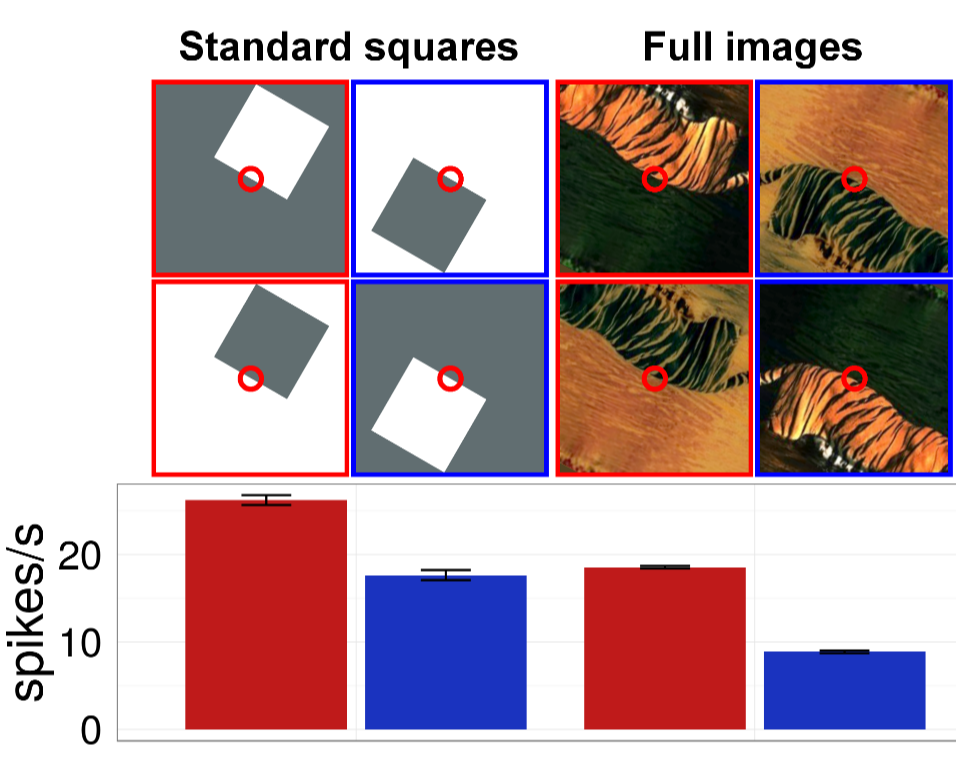
\includegraphics[width=.4\textwidth]{figs/bos_naturalimages_clipped}
  \caption{BOS signal in natural images} 
  \vspace{-15pt}
  \label{fig:NaturalImages}
\end{wrapfigure}
%\end{figure}

\textbf{Model predictions.}
I predict that V1 responses to closed contours will be higher than to
open contours. Although there is psychophysical evidence for the
increased detectability of closed contours versus open
contours~\citep{Kovacs_Julesz93}, to the best of my knowledge, there
are no electrophysiological studies comparing V1 responses to these
two types of contours. To study this
%
using a modeling approach, 
I will create artificial images that either have a single open contour (similar to the experiments in~\citet{Chen_etal14}), or a square object which has a closed contour
(see "Preliminary results"). Due to the feedback from object grouping
cells which are selective for a cocircular arrangement of contours, a
V1 neuron along the closed contour will receive greater feedback and
show enhanced activity. Models without feedback would treat each edge
of the square as a separate contour, such that the activity of a V1
neuron along an edge of the square would not be more active than if
four separate contours were shown. {\em These two types of models make very different predictions, which can be used to test the models.}

\begin{wrapfigure}{r}{.45\textwidth}
%\begin{figure}[h]
  \vspace{-10pt}
  \centering 
  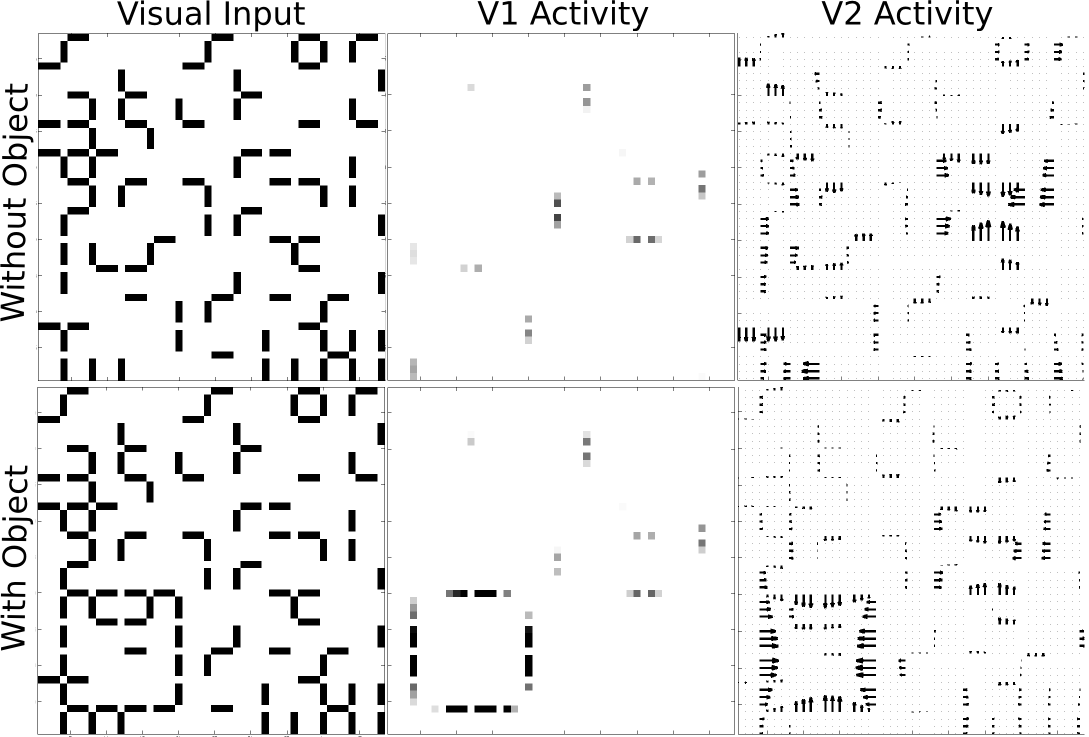
\includegraphics[width=.45\textwidth]{figs/contour_revised}
  \caption{Object contour grouping} 
  \vspace{-5pt}
  \label{fig:ContourGrouping}
\end{wrapfigure}
%\end{figure}

I also predict that attention biases competition between
multiple objects and selectively enhances V1 responses on the attended
object while suppressing responses on the unattended object. I will use a stimulus where two square objects are present
(similar to \citep{Qiu_etal07}), which activate multiple grouping
neurons at the level of V4. I will then study how attention directed
to the grouping neuron corresponding to the attended object modulates
the responses of V1 neurons on both objects. 
%Selection of an object
%contour among multiple contours has not yet been tested
%experimentally, and
My model will clarify the degree to which selection of an object contour among multiple contours
%this
%process
occurs pre-attentively and the degree to which this process
requires top-down attention. I also predict that attention will change
response bias: When attention is applied, the subject will
be more likely report detecting a contour due to the increased
activity of grouping cells in V4 which represents object information,
as well as the increased feedback to V1 which biases the activity of
V1 neurons.

\textbf{Preliminary results.} I extended an existing grouping model~\citep{Mihalas_etal11b} by adding feedback to the V1 neurons that encode edges in the visual input. Figure~\ref{fig:ContourGrouping} shows preliminary results from these model simulations. 
The left column shows the visual
input, the center column shows the response of V1 neurons pooled
over both orientations, and the right columns shows the response of BOS V2 neurons. Darker colors indicate higher activities for the V1 neurons, while for the V2 neurons, the direction and magnitude of the arrows indicate the side-of-figure and strength of the border ownership signal, respectively.
The top row shows a noise pattern where no object is
present, while the bottom row shows the same noise pattern with a
square object located in the lower left. Object grouping neurons in V4
(not shown)
are more activated in the presence of an object, and as a result, send
greater feedback to V1 and V2 neurons, highlighting the contour of the
object and assigning correct border ownership along the contour.
%This feedback interacts with local lateral connections to
%enhance the object while suppressing the background. 
%This mechanism
%can thus select objects in highly cluttered visual
%scenes.
%Attention acting at the level of grouping neurons may further
%increase response enhancement of the object contour (not yet
%tested).
My model's ability to perform both contour enhancement and border ownership assignment with the same set of parameters increases my confidence that it describes the underlying grouping mechanisms.

%My model will avoid overfitting to a single experiment by also reproducing previous border ownership findings~\citep{Qiu_etal07}. Measuring the responses of BOS neurons under different conditions will confirm these results.
%en why not show that in an additional column in the figure?

\subsection{Neural circuits underlying surface grouping (Aim 2)} 
\textbf{Rationale.} Very little is known about how the brain 
represents
surfaces.
%en cut to save space:
%, so the model will provide valuable insight
%into the neural circuits involved in this process. 
I propose that
grouping neurons in V4 respond to surfaces defined by 3D
objects. Feedback from these grouping neurons not only enhances the
responses of disparity-selective neurons that are part of the surface,
but also sharpens their disparity tuning.
 
\textbf{Model design.} In the surface grouping model,
feature-selective neurons respond to binocular disparity (one of many
possible depth cues) instead of orientation.  I used eight
orientations in the contour grouping model, but many more disparity
values are needed to represent smoothly-varying 3D objects and
surfaces. This potentially leads to the ``curse of dimensionality,''
as many neurons are needed for this type of representation. In order
to avoid this problem, I will build on previous work originally
developed to explain coordinate transformations in the motor system
\citep{Salinas_Abbott95, Pouget_Sejnowski97b}. In this framework,
retinotopic RFs in parietal cortex exhibit gain-field modulation in
eye position. These RFs form a complete basis set of the space spanned
by retinal coordinates and eye coordinates, enabling transformations
between eye-centered and head-centered coordinate systems. The weights
of these transformations can be learned by a simple Hebbian-type rule
or supervised learning~\citep{Salinas_Abbott95}. {\em I propose that
  these same ideas can be employed to represent disparity in a much
  more efficient way than by representing each disparity value with a
  dedicated neuron.} The mathematics (including learning rules) are
identical to those used for coordinate transformations, except that
the eye position variable is replaced by binocular disparity.

\begin{wrapfigure}{r}{.4\textwidth}
%\begin{figure}[h]
  \vspace{-20pt}
  \centering 
  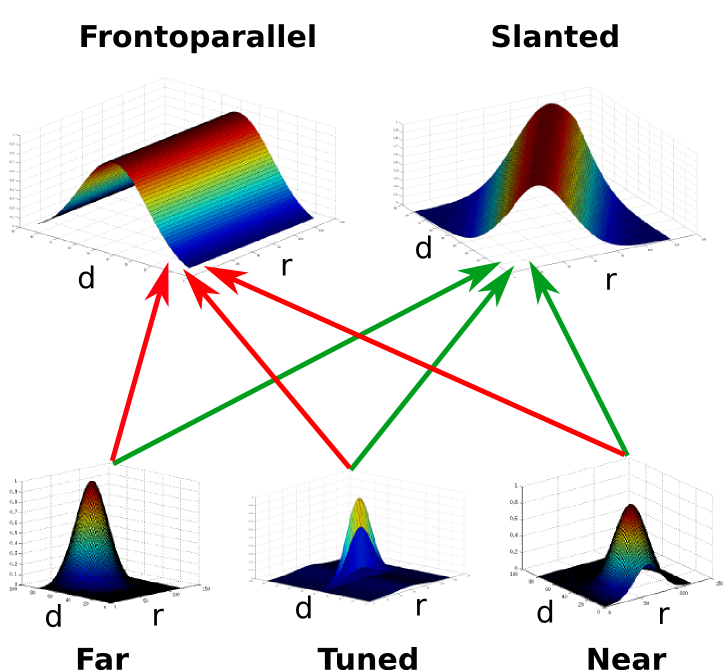
\includegraphics[width=.4\textwidth]{figs/basisfunc}
  \caption{Basis functions for surfaces} 
  \vspace{-15pt}
  \label{fig:BasisFunctions}
\end{wrapfigure}
%\end{figure}

Supporting these ideas, previous experimental results have shown that
V2 neurons have gain field-like properties, with their responses to
stimulus orientation depending nonlinearly on
disparity~\citep{vonderHeydt_etal00a}. Disparity-selective neurons
then form a basis set spanning retinotopic position (a two-dimensional
vector $r$, only one coordinate of which is shown for ease of visualization)
and disparity ($d$), which can be used to create any object or surface
in 3D space (Figure~\ref{fig:BasisFunctions}). For example, using the
same basis set of disparity-selective neurons (only three neurons are
shown here), an optimal set of weights can be found which define
different 3D surfaces in space. Arrows in the figure indicate weighted
connections that combine the activity of these basis function units
into new RFs (frontoparallel plane, left and slanted plane, right). In
my model, neurons with RFs as in Figure~\ref{fig:BasisFunctions} group
the features of an object or surface in 3D space, {\em in complete analogy
to the grouping mechanisms in 2D.}

In this model, I will include visual areas V2 and V4. There is
evidence that BOS 
neurons in V2 respond to contrast-defined and disparity-defined edges,
combining both cues to determine border
ownership~\citep{Qiu_vonderHeydt05}. I hypothesize that V4 contains surface grouping
neurons, which group together objects along a surface with a preferred
depth and slant, and also feed back to the corresponding V2
neurons. Lateral connections exist between different
disparity-selective neurons within a retinotopic location in V2, which
refine the feedback signal received from grouping neurons. The
strength of these lateral connections is determined by the Pearson
correlation of the feedforward disparity tuning
curves~\citep{Samonds_etal13}. Similarly, lateral connections also
exist within V4 to mediate competition between grouping neurons
responding to different surfaces. The other model implementation
details are the same as for the contour grouping model. 

\textbf{Model validation.} I will validate my model using
psychophysical results from a study showing that the local 3D
orientation of objects along a surface influences visual
search~\citep{He_Nakayama95}. Changing the local 3D orientation of
objects along the surface changes the amount of feedforward input
surface grouping cells in V4 receive, which will also affect the
amount of feedback they send back to V2 (see "Preliminary results"). 

\textbf{Model predictions.} Previous studies have not examined whether feedback enhances responses of neurons in V2 coding for the same surface or whether feedback sharpens disparity
tuning in V2.
In order to quantify changes in disparity tuning, I
will use the measure of sample skewness, which is the third
standardized moment of a distribution~\citep{Samonds_etal13}. Sample
skewness can be directly computed from the mean firing rates $f(d) $
for each preferred disparity $d$ of the model neurons. I predict that
V2 neurons that
are part of well-formed surfaces (\eg frontoparallel or slanted) will show higher activities due to
increased feedback from grouping neurons. Secondly, I also predict
that with attention, the firing rate of V2 neurons that are part of
the attended surface will increase. Finally, I can examine the effect
of attention on disparity tuning. As recurrent connections have been
shown to be important for sharpening of disparity tuning in
vivo~\citep{Samonds_etal13}, I predict that attention will further
sharpen disparity tuning in a surface-based manner. 

\textbf{Preliminary results.} Figure~\ref{fig:Nakayama} illustrates the experimental paradigm of~\citet{He_Nakayama95}. The top
\begin{wrapfigure}{r}{.4\textwidth}
%\begin{figure}[h]
  \vspace{-10pt}
  \centering 
  \includegraphics[width=.4\textwidth]{figs/nakayama_v2}
  \vspace{-30pt}
  \caption{Attention to surfaces} 
  \vspace{-15pt}
  \label{fig:Nakayama}
\end{wrapfigure}
%\end{figure}
row in A shows schematically the 3D search arrays used in the experiment. Subjects had to search for a target in the middle disparity plane. In A-a, objects are aligned in the search plane while in A-b and A-c, they are slanted out of the plane. The middle row in A shows reaction times, which are significantly shorter when the objects are coplanar with the search plane (A-a) than when they are misaligned (A-b and A-c). The reason for this trend is clear from my model. I postulate that there are dedicated surface grouping neurons which organize the visual scene into oriented planes, such as those shown at the top of Figure~\ref{fig:BasisFunctions}. Attention directed to the grouping neuron with frontoparallel orientation selectively feeds back to all objects on the corresponding surface. Among the objects in the middle frontoparallel plane, the target has a unique color, allowing for efficient search. In A-b and A-c, the objects are no longer coplanar with the attended grouping neuron, which results in reduced feedback and longer reaction times. This result is not restricted to frontoparallel planes, as similar results were also found for slanted planes (B). The bottom rows in A and B show results of simulations of these experiments, which are now published~\citep{Hu_etal15a}. The model generalizes a simple stereomatching model~\citep{Marshall_etal96} to allow for top-down attentional selection of specific surfaces by increasing the activity of the corresponding grouping neuron. Attention to grouping neurons is then able to select sets of objects organized in planes. Reaction times are difficult to simulate, therefore I plot the mean increase in disparity-selective neuron activity on the surface due to attention, which is assumed to be inversely proportional to reaction times.

\subsection{Potential problems and alternative strategies}
%think of more specific risks- talked about location of grouping neurons for SA2?
The general risk of the proposed experiments is low because the
methods and techniques used have been honed in the mentor's lab for
years. Surface grouping neurons have not yet been found, although some
neurons in parietal cortex show sensitivity to the 3D orientation of
planar surfaces~\citep{Rosenberg_etal13}. I will adjust my models
accordingly to reflect any new physiological findings. To mitigate the
risk of a negative result,
%en seems a bit of an unfortunate formulation: a negative result can
%be useful, too. You are testing hypotheses, and it should be OK if
%the test of the hypothesis shows that it is wrong...
 I propose here two sets of experiments,
with the first (Aim 1) a direct derivate of previous contour-based
models developed in the sponsor's lab, and the second (Aim 2) a bit
more adventurous involving 3D surfaces, which to my knowledge have
never been studied in a quantitative, neurally plausible model. It should be noted that negative results can also be informative and useful for falsifying the grounding assumptions of our models.
 
\subsection{Timeline} Work on Aim 1 will take place during the first year. Modeling efforts will first seek to reproduce previous experimental findings, then move on to testing model predictions. Work on Aim 2 will begin in the second year.
%, concurrent with modeling experiments involving the contour grouping model.
Final analyses and publications related to the research will be completed by the end of the second year.

\clearpage

\section*{Path to Graduation}

\textbf{Expected Time to Graduation.} I expect to graduate in two years (approximately May 2017). The milestones I have set for myself in order to reach this goal are to: 1) successfully propose my thesis, 2) publish on several of my research-related "side projects", and 3) complete work on the specific aims related to this proposal, while also publishing on these results. Working towards these milestones will take up the majority of my time. I hope to be able to successfully write up and defend my thesis in the remaining time.

\textbf{Coursework.} I have already completed the required coursework for my program, but will continue to expand my current neuroscience knowledge by auditing graduate classes relevant to my research. I plan to take a "Computer Vision" course, which will introduce me to the computer vision approaches to grouping and segmentation that are the focus of this proposal. I also plan to be an active participant and presenter in the departmental journal club that discusses current neuroscience publications (''Readings in Systems Neuroscience'').

\textbf{Presentations, Seminars, and Meetings.} I will be attending many seminar series throughout the award period, including our departmental colloquium series (the ''Bodian Seminar''), which is held weekly at the Mind/Brain Institute. I will also attend relevant talks (related to my current proposal) at the medical school's Neuroscience Seminar Series and through the Brain Science Institute's ''Brain Night''. Finally, I will connect with other scientists from around the world by attending and presenting at relevant conferences, including the annual Society for Neuroscience and Cosyne meetings.

\textbf{Manuscript and Grant/Fellowship Submissions.} I have recently presented and published my research at the IEEE Conference on Information Sciences and Systems (CISS)~\citep{Hu_etal15a}. I am currently preparing another manuscript related to how the addition of depth information to a proto-object based saliency model improves the model's ability to predict perceptual saliency (eye fixations) under both 2D and 3D viewing conditions. I am also currently collaborating with a former post-doc in our lab on a disinhibition-based model of grouping to explain recent firing rate and spike synchrony experimental results, which I hope to publish in the near future. In terms of grant/fellowship submissions, I have re-submitted an NIH F31 NRSA fellowship in the last funding cycle (April 2015), the focus of which is largely covered by this proposal.

\clearpage

%\section*{Activities Planned Under this Award}
%
%\textbf{Research Training.} Under this grant proposal, I plan to first
%and foremost become fully trained in computational modeling as a tool
%for understanding neural circuits in the brain. I will also be trained
%in computational analyses of modeling data in order to relate these
%results to previous physiological findings. Such training will take up
%the majority of my time ($\approx$ 80\%). During the first year of the
%award, I will begin by building a model of contour grouping
%constrained by recent physiological data~\citep{Chen_etal14}. I will
%work closely with both Dr. Niebur and Dr. von der Heydt to ensure that
%the model I propose is computationally and neurophysiologically
%feasible. I will first use my model to reproduce experimental results,
%which show different, but cooperative responses in V1 and V4 neurons
%during contour grouping. I will also extend
%    my model to natural images and quantify its performance by
%    comparing my results to human-generated ground truth
%    data. With the help of Dr. Niebur, I will also learn
%how to perform a global sensitivity analysis on the parameters of the
%model. Next, using my model, I will seek to answer the research
%questions that I have proposed, mainly related to how 
%attention interacts with the grouping
%    circuit in an object-based manner to both bind together
%    feature-selective neurons as well as enhance their
%    activities.
%% feedforward, feedback, and lateral connections interact in neural circuits. By changing the respective weights of each of these types of connections within the circuit, I can study their effect on contour grouping, and ultimately object perception.
%Dr. Niebur has previously proposed that top-down attention taps into
%the same neural circuit used to generate border ownership, and
%similarly, I can test whether attentional mechanisms also use the
%contour grouping circuit to modulate the responses of early visual
%neurons that are part of an object
%    contour. During the second year of this grant, I will
%extend the 2D contour grouping model to grouping of
%3D surfaces. Dr. von der Heydt is an expert in
%binocular vision, having extensively studied disparity-selective
%neurons in visual cortex throughout his academic career. With the
%addition of a spatial dimension in depth (along with 2D retinotopic
%space), the complexity and dimensionality of the system under study
%greatly increases. Dr. von der Heydt's insight into efficient neural
%coding of disparity will be particularly useful as we have continued
%discussion about how neural circuits may use basis functions to transform depth
%information into 3D planar surfaces that organize the visual
%scene. The Niebur lab has a long-standing record of creating simple,
%yet informative models of vision that reproduce physiological results
%and also make nontrivial predictions that can later be tested
%experimentally. If the opportunity presents itself, I will also
%collaborate with Dr. von der Heydt to experimentally test some of the
%predictions made by my models. Overall, Dr. Niebur and I believe that
%this training plan will help me develop into an independent scientist
%skilled in the computational modeling of neural circuits, particularly
%in the study of how attention and object representations interact in
%early vision.
%
%\textbf{Coursework.} I have already completed the required coursework for my program, but will continue to expand my current neuroscience knowledge by auditing graduate classes relevant to my research. I also plan to take a "Computer Vision" course, which will introduce me to the computer vision approaches to grouping and segmentation that are the focus of this proposal. I was the teaching assistant for the "Networks" course during the fall semester, which means that I have now completed all of my teaching requirements. I plan to be an active participant and presenter in the departmental journal club that discusses current neuroscience publications (''Readings in Systems Neuroscience''). I will also participate in weekly lab meetings, where I will have the opportunity to present on my research progress and receive constructive feedback from my colleagues. Such academic endeavors, until the final year, when I will be finishing up computational analyses and preparing publications, will take up all additional time while not working directly on the proposed experiments.
%
%\textbf{Presentations, Seminars, and Meetings.} I will be attending many seminar series throughout the award period, including our departmental colloquium series (the ''Bodian Seminar''), which is held weekly at the Mind/Brain Institute. I plan to invite a speaker related to visual attention for a Bodian Seminar next year (students are encouraged to invite one speaker each year). I will also attend relevant talks (related to my current proposal) at the medical school's Neuroscience Seminar Series and through the Brain Science Institute's ''Brain Night''. Finally, I will connect with other scientists from around the world by attending and presenting at relevant conferences, including the annual Society for Neuroscience and Cosyne meetings.
%
%\textbf{Outreach Activities.} I will also attend events through the School of Education's Neuro Education Initiative. I plan to be involved with this organization and present relevant research on attentional mechanisms related to vision and object perception. I believe educators will find this information useful and insightful for their daily work.
%
%\clearpage
%
%\section*{Doctoral Dissertation and Other Research Experience}
%My research experience began in Dr. Aaron Batista's lab at the University of Pittsburgh, where I completed undergraduate research on sensory-motor integration. Working with a graduate student, I studied how monkeys are able to adapt their arm movements in response to various types of sensory feedback. Users of neural prosthetics currently only receive visual feedback about their limb movements, which is relatively slow and limiting, while the role of proprioceptive and tactile feedback has largely been unexplored. I was interested in comparing the reaction times of monkeys in a reach redirection task which required them to change the direction of their arm movements in response to either a visual cue or a vibrotactile cue placed on the skin. Single unit recordings from primary motor cortex were also made to test whether there was a neural correlate of these reaction time differences. Our hypothesis was that reach redirections due to the vibrotactile cue would be faster than the visual cue, suggesting that forms of proprioceptive feedback are important for optimal control of neural prosthetics. For this project, I was responsible for designing an automated algorithm that could detect the time point at which reach trajectories diverged from their original path by looking at both the recorded position and velocity movement traces. I also helped out with hardware design related to the experiments, including building a photodetector circuit for measuring display screen latencies, as well as designing a cost-effective motion capture system using Nintendo Wii-motes. I was also given the opportunity to help with training monkeys on the task, as well as doing some single unit recordings. These experiences sparked my interest in systems neuroscience, and exposed me to the richness of the research questions that could be asked about the brain.
%
%During my first year at Johns Hopkins University, I briefly explored research in medical robotics, as I was interested in how engineering applications could improve the quality of life of patients. I worked in the lab of Dr. Russell Taylor, in the Computer Science and Radiology departments. I helped design a novel force sensing tool that could be used with a robotic system for microsurgery within the eye. The robotic system, named the Eye Robot, was designed to improve patient outcomes by reducing surgeon hand tremor when using surgical tools and providing force feedback to the surgeon. Force feedback is important because it allows the surgeon to know when a tool is about to touch important structures within the eye (e.g. the retina) that might be damaged if excessive force is used. I designed the protocol for an IRB-approved experiment involving human subjects to assess their ability to perform a mock procedure without the use of the Eye Robot. Using an ex vivo model of the retina, subjects were asked to try and penetrate a blood vessel and fill it with a high-contrast fluid, mimicking an actual retinal microsurgery operation. During each trial, subjects' reaction times, success rates, and damage to the surrounding tissue were recorded. I found that subjects performed the experiment faster and with less trauma when they used the Eye Robot compared to freehand, when they were unassisted by the robot. I was also able to ask two practicing retinal microsurgeons to test the tool in vivo, by performing a similar experiment on anesthetized rabbits at the medical school. The lab is still collecting data from subjects performing the experiments, and we hope to publish a paper on our results soon. I independently created the experimental task used to measure human performance and was aided in the collection of data with the help of two undergraduate students.
%
%I also performed research in Dr. Ed Connor's lab at the Mind/Brain Institute during my first year in the graduate biomedical engineering program. I was interested in examining whether higher visual areas could jointly code for object identity and value. Rather than simply acting as one stage in the feedforward visual hierarchy that ultimately encodes object identity, I was interested in whether the responses of neurons in inferotemporal cortex (IT) could also be modulated by the relative value of an object. IT neurons receive many projections from prefrontal cortex, which is known to be a locus for value and decision making. My idea was to train monkeys to choose between two different objects, whose relative value differed based on a reward rule involving their stimulus features. Each object would be composed of various stimulus features, and the monkey would have to learn to associate conjunctions of these features, rather than individual features themselves, with a reward. This is a natural process, as we holistically evaluate objects for aesthetic beauty and value (e.g. faces with the conjunction of eyes, nose, mouth, etc.) I hypothesized that after learning, the responses of neurons in IT would not only encode object identity, but also object value as well. I was interested in tracking neural tuning changes in IT throughout the learning process, as the neurons might shift from only coding object identity to a hybrid coding of object identity and value. I began by designing the set of visual stimuli and reward rules to be used in the experiment, and started to set up a simple human psychophysics experiment using the stimuli. Although we were not able to collect any data, we believe that human subjects can quickly learn to discriminate between the value of two objects. I conducted this project with the help of Dr. Connor and another graduate student in the lab, who helped guide me through the initial stages of the work.
%
%Finally, I began my current research in Dr. Niebur's lab almost three years ago. I began by working on extending a previous neural model for assigning border ownership to edges along an object. The model used grouping neurons which integrate global context information about the object and then feedback to the corresponding edge neurons~\citep{Craft_etal07}. The aim of my study was to determine whether the same neural circuit used for 2D shapes could also be used to explain grouping of  3D surfaces. I first tested my new model on simple 3D shapes (e.g. cubes, pyramids, etc.), and as I predicted, it was able to correctly assign the direction of border ownership for a surface patch using global information about the object. Next, I was interested in whether lateral inhibition between grouping neurons representing the parts of a surface could be used to form the 3D medial axis of an object. The medial axis provides a topological, skeleton-like structure for any object, which is a useful shape representation because it allows for recognition of the same object from many different views. Neurons in inferotemporal cortex have been found to encode the 3D medial axis of objects, along with surface patches along the object~\citep{Hung_etal12}, consistent with the grouping neurons I proposed in my model. I tested my model on publicly available 3D object models (Princeton Shape Database), and began work on classifying different object classes using their 3D medial axis structure. More recently, I extended a neural model for stereomatching~\citep{Marshall_etal96} to explain psychophysical results related to directing attention to 3D surfaces~\citep{He_Nakayama95}. In my model, surface grouping neurons modulate the activity of disparity-selective neurons through feedback. Attention is able to select a specific surface grouping neuron, which then enhances the activity of disparity-selective neurons on the attended surface. I was able to present my work at the IEEE CISS conference, which also resulted in a publication~\citep{Hu_etal15a}.
%
%%We also began discussion about the feasibility of my model with scientists working on the hippocampus, where perirhinal cortex and lateral entorhinal cortex may contain such grouping neuron representations. These two areas in the hippocampal network contain neurons which show much more object-related tuning, rather than place-related tuning, and may be important for the memory and representation of object landmarks when navigating different environments.
%
%The proposed research plan will add to this research experience by building on my foundation in computational modeling of vision. Following this training plan, I will be completely proficient in creating physiologically-constrained models of neural circuits and using these models to reproduce existing experimental results. In addition, I will be able to use the models that I have created to make interesting predictions of phenomenon that have not yet been tested experimentally, providing a valuable tool for testing various computational hypotheses about the neural circuits in the brain. Throughout this proposed research, I will be working closely with a computational neuroscientist (Dr. Niebur) and a neurophysiologist (Dr. von der Heydt), which will help to focus my models on the important research questions that have not yet been asked. I am currently able to simulate simple network models of neural circuits, and comfortable with the mathematics and practical implementation of these simulations. Following this training plan, I will be well versed in the simulation of small-scale, quantitative firing rate models that involve detailed connections between multiple cortical areas, and also the computational analyses of the resulting data in relation to previous experimental findings. I will also gain experience in applying computational models to natural images, which are inherently complex due to their high dimensionality. I will also have worked on early object representations in two different systems (2D contour grouping and 3D surface grouping), which will be useful as I go on to study other systems. My dissertation project will center around the experiments in this proposal, exploring the neural circuits underlying early object representations and how attentional mechanisms interact with these circuits. The latter goal includes exploring how attention interacts with early feature representations to modulate their responses, as well as how attention may mediate selection between competing objects.
%%I will also examine the role of different types of connections (feedforward, feedback, and lateral) within the cortical circuit, and study their effect on perception by changing the corresponding parameters in the model.
%
%\clearpage
%
%\section*{Equipment}
%
%The Niebur lab has a cluster of over 20 state-of-the-art computers running Linux which are connected to each other and to the internet by fast ethernet. They can be used individually, as a distributed computer (through Beowulf, PVM etc), or by using our custom-written parallel event-driven neuronal simulator~\citep{Mihalas_etal11a}. Each student and postdoc has a desk with one or multiple LCD screens. Color printing facilities are provided by the Institute, as is technical support through a full-time systems administrator.
%
%Electronics and machinist staff (three full time, one part-time) and workshops are shared with other labs in the Mind/Brain Institute.
%
%\clearpage
%
%\section*{Goals for Fellowship Training and Career}
%My academic and professional goals are to perform graduate and postgraduate work in computational neuroscience research, particularly related to vision and attention. I hope to then teach neuroscience in a university setting while continuing to pursue this type of research. I wish to explore the neural circuits underlying object vision, which will hopefully provide us with a computational and theoretical framework for understanding neural circuits in the brain. Computer vision research has given us many practical applications, yet few fundamental guiding principles about the algorithms or computations involved in vision. I firmly believe that studying the neural circuits underlying vision will greatly aid us with this understanding. This is why I am excited about this proposal. It will help me understand how the brain's neural circuits form early object representations which efficiently organize the visual scene, and allow me to test a mechanism by which attention, which is not currently considered in computer vision, can modify these object representations. I hope to continually use computational modeling techniques to build physiologically realistic models of the brain that not only reproduce previous experimental findings, but can also give us testable predictions and new directions for research. In the future, I hope to continue on in my collaboration with both computational and systems neuroscientists, which will allow for cutting-edge partnerships and discoveries. Under this proposal, I would become fully skilled in running small-scale network simulations of neural circuits that can be applied to both artificial and natural images. In addition, I would feel comfortable building new models, running simulations, and performing computational analyses of the resulting data on my own.
%%, and would feel comfortable building new models and running simulations on my own.
%%In addition, I would be trained in computational analyses of the resulting data.
%I believe that by being trained in these computational tools early on in my graduate education, I will be able to utilize them while conducting research in my own laboratory and fully understand their strengths and limitations in different settings.
%
%I found that during my initial training in neuroscience, I was most interested in the underlying neural circuits that generate the experimentally observed neural responses and behavior. In the era of big data, scientists continue to perform well-designed experiments that give us more facts about the brain, but fundamental neuroscience principles upon which we can hang these facts and better understand how the brain processes and transmits information are still lacking. How does the brain integrate the different streams of information carried by
%%Why is it that every part of cortex has 
%feedforward, feedback, and lateral connections and make use of them for visual processing?
%%How does the brain use each of these types of connections for information processing in neural circuits?
%What is the role of attention? Network-level neural simulations constrained by physiological data will allow me to easily test different computational hypotheses. By building models which incorporate these different types of connections as well as attentional input,
%%varying the parameters in the model corresponding to different types of connections or attentional input,
%I will be able to offer a simple, phenomenological explanation for how the underlying neural circuit generates the observed neural responses. My goal is to understand how the brain functions at the level of neural circuits and how this function is related to perception and behavior. This project affords me the opportunity to study these questions in detail.
%
%I believe that this project will allow me to study the neural circuits involved in vision from several angles. After completing this training plan, I will have the skills and knowledge to create future studies exploring other issues in visual attention, as I am already realizing future experiments that need to be completed in the field. A full explanation of how the brain's early feature representations interact with attentional mechanisms can only be achieved with the collaboration of different levels of analysis. If we are to truly understand the function of neural circuits, we must know how they interact at the cellular, systems, and behavioral level. Therefore, I plan to keep up-to-date with new findings in neuroscience research that span these multiple levels (including, for example, the identification of new interneuron cell types that might play specific roles in neural circuits), and hope in the future to collaborate with scientists who study neural circuits at this level.
%
%I plan on conducting research that has relevant clinical applications to vision and attention. For example, deficits in object-based attention have been implicated in neglect, where patients are not aware of the features or parts of an object. I wish to explore how the neural circuits underlying vision in normal, healthy patients differ from those that underly different disease states, with the hope that neuroscience findings will enhance our rehabilitation and treatment efforts. Furthermore, I believe that understanding how attention modulates early feature representations extends beyond vision. The brain may also use similar neural circuits to organize incoming auditory, tactile, or olfactory information into object representations that can then be selected by attention. Again, I believe that the combination of computational modeling and close collaboration with neurophysiologists will be essential for helping me achieve my research goals.
%
%\clearpage
%
%\section*{Facilities and Other Resources}
%
%The 800 square foot computational neuroscience laboratory headed by Dr. Niebur houses a cluster of about two dozen fast workstations (single or multi-core, single or multi-processor), all running Linux and all interconnected by fast ethernet. Machines are flexibly organized into a fully parallel cluster using the Parallel Virtual Machine architecture or our custom-written spiking Event Related Simulation Tool. All graduate students and postdocs work in one laboratory to enhance interactions. There is a separate office for the PI, and another office hosts an invited professor (currently Dr. Kazuyoshi Tsutsumi from Ryukoku University, Japan). Each student or postdoc has a desk with a Linux workstation (all connected with each other and the computational cluster by fast ethernet) with one to three computer screens. Secretarial support is provided by four staff and one chief administrator, all full time, shared between a total of ten faculty in the Mind/Brain Institute.
%
%\textbf{Scientific Environment.} The Johns Hopkins University provides a unique environment for the proposed research. The Mind/Brain Institute has four laboratories that study the neural mechanisms of visual and tactile perception, cognition, and motivational control of behavior. Other laboratories affiliated with the Biomedical Engineering Department study auditory perception with similar methods. All these groups meet regularly and have lively interactions. The technical support is excellent. There is also a multitude of interactions between theoreticians. For instance, Dr. Niebur runs (together with Dr. Kechen Zhang from the BME department) the university-wide Working Group for Computational Neuroscience of the Brain Sciences Institute. Two weekly departmental colloquia (one in the Mind/Brain Institute, run by Dr. von der Heydt) and two weekly departmental journal clubs (one in the Mind/Brain Institute), among many other events, provide an intellectually rich environment for students and faculty.
%
%\clearpage
%
%\section*{Project Narrative}
%
%We wish to understand how object contours and surfaces are grouped together using computational models of the neural circuits underlying vision and attention. Specifically, we are interested in how different cortical areas and types of cortical connections contribute to our perception of objects and our ability to attend to objects. Our findings will describe healthy brain function in adults with normal vision, but may also guide treatments or rehabilitation in the diseased brain, such as for cases of object-based neglect.
%
%\clearpage
%
%% Please edit Project Summary section!! bh
%
%\section*{Project Summary/Abstract}
%Funds for this proposal will be used to train the applicant in
%computational modeling of the neural circuits underlying object
%vision. The proposed modeling experiments will address how visual
%features are grouped into 2D and 3D object representations. In
%\textbf{Aim 1}, we will model the neural circuits underlying grouping
%of 2D object contours. We test here whether a similar neural circuit
%is used to group together object contours and
%    to perform segmentation and figure-ground assignment in artificial
%    and natural images. We believe that feedback from
%higher cortical areas is critical for shaping early object
%representations, in constrast to
%most traditional models of vision, which are purely feedforward.
%We will extend our model to explain segmentation and figure-ground
%assignment in natural images, which has not yet been studied. We will
%also use our model to make experimental predictions that have the
%potential to falsify our model. One prediction is that object-based
%attention uses the same grouping circuit to mediate competition
%between different objects during the selection process.  
%Previous studies on the neural coding of border ownership have
%identified a plausible network architecture that involves populations
%of grouping neurons which integrate global context information about
%an object and send feedback connections back to feature-selective
%neurons that are part of the object, modulating their activity.  We
%are also interested in how the brain represents groups of objects
%along 3D surfaces, which may be ecologically important for tasks such
%as locomotion and reaching. In \textbf{Aim 2}, we will build a model
%of surface grouping in analogy to the contour grouping model above by
%using basis functions, which have many
%    computational advantages and are theoretically
%    tractable. We are interested in the interaction between
%disparity-selective neurons in early visual areas and grouping neurons
%which code for planar surfaces composed of objects. We hypothesize
%that surface grouping neurons are located in V4. 
%%en although the neurons that you list earlier as candidates were
%%found in CIP...
%The model makes three
%testable predictions. First, we hypothesize that disparity-selective
%neurons show enhanced activity when they are part of a well-formed
%surface because they receive greater feedback from grouping
%neurons. Second, we propose that attention to the surface further
%increases the activity of disparity-selective neurons using the same
%neural circuit. Finally, we hypothesize that attention not only
%increases the activity of these neurons, but also sharpens their
%disparity tuning. Previous findings have shown that local recurrent
%connections can account for the sharpening of disparity tuning seen in
%vivo, but the effect of attention was not examined. Our findings will
%give us insight into brain function under normal vision, but may also
%provide us with information about which parts of the neural circuit
%are deficient in various disease states, such as for object-based
%neglect. Our results will also give us a better understanding of the
%fundamental principles governing neural circuits in the brain,
%specifically how different cortical areas and cortical connections
%work together to process and transmit information in the brain.
%
%\clearpage
%
%\section*{Respective Contributions}
%
%Dr. Niebur and I worked together to create the general outline of this
%proposal, with helpful input from Dr. von der Heydt as well. I
%expressed interest in studying the neural circuits underlying early
%object vision, and sought to understand how these circuits might be
%used in the context of contour grouping and surface grouping. I
%conducted background research on this idea to see if it was feasible
%based on previous work. Dr. Niebur pointed me to various computational
%tools and analyses that will prove useful in completing the proposed
%research. Dr. Niebur also guided me on approaches to creating
%physiologically-constrained models, while I worked out the specifics
%of implementing these models and identifying the relevant research
%questions that could be asked using these models. We have worked
%together to create a plan in which I can learn about both the
%neurophysiology and modeling techniques needed to describe neural
%circuits and relate them to perception. I have personally written the
%entire proposal with Dr. Niebur's input and commentary throughout the
%editing process. Even with our close collaboration, Dr. Niebur has
%given me the independence to create a unique training plan that serves
%my interests. We hope that this balance in contributions is evident in
%the application. 
%
%\clearpage
%
%\section*{Responsible Conduct of Research}
%
%I have completed a two-semester research ethics course through the School of Medicine, entitled ''Introduction to Research Ethics 1 and 2.'' This course involved lectures on various topics, followed by faculty-led small group discussions. During these small group discussions, several real-life scenarios were presented using role play, through which faculty mentors guided discussion about the ethical course of action in these situations. During the fall, the course covered topics related to scientific integrity and scientific misconduct, academic integrity and cheating, managing data, mentorship, and plagiarism. During the spring, the course covered topics related to being a member of the scientific community, intellectual property, animal research, and human subjects protection. In addition to this course, I have completed an online animal training course (08/15/11) through the Johns Hopkins Animal Care and Use Committee (IACUC). I have also completed an online training module (08/15/11) on conflicts of interest offered through the School of Medicine. Finally, I have completed an online course (11/15/11) for conducting ethical research and protection of human subjects that is approved by Johns Hopkins' local review board (IRB). This included training related to health information privacy (HIPAA). During my training, I plan to meet with my mentor bi-monthly to discuss ethical issues. The biomedical engineering department also offers an ethics course related to engineering innovation, which I plan to take this year. This course is essential for a biomedical engineer like me, who must be able to understand and clearly communicate how my research impacts society. The course description is given below.
%
%\textbf{Ethics of Biomedical Engineering Innovation.} Engineers confront problems and make decisions that hold long term social consequences for individuals, organizations, communities, and the profession. For biomedical engineers, these decisions may relate to: inventions such as medical devices and pharmaceuticals; neural prosthetics and synthetic biological organisms; responsible and sustainable design; availability of biotechnology in the developing world. Using a combination of cases, fieldwork, and readings, we examine the ethical issues, standards, theory and consequences of recent and emerging engineering interventions as a way to understand the profession and to form a basis for future decisions. In addition students will learn and practice multiple forms of communication, including oral, visual and written rhetoric.  A particular focus will be communication targeted to different stakeholders including other professionals and the public. Students will apply good communication principles to the discussion of biomedical engineering ethics, develop their own ethical case studies, and participate in group projects to aid ethical decision-making, and to improve communication of complex biomedical ethical issues to others.
%
%\clearpage
%
%\section*{Selection of Sponsor and Institution}
%
%The Johns Hopkins Biomedical Engineering department is consistently ranked as the top program in the country and has continually produced exciting breakthrough research. The department is well known for collaborations that span many different disciplines, which is what drew me to the institution. Here, there is truly an environment of scientific partnership to create new ideas and discoveries. The department is present on both the medical school campus, where most cellular and molecular research takes place, and the ``Homewood campus,'' which houses the School of Arts and Sciences and the School of Engineering and where most computational and systems research takes place. Students are encouraged to explore both areas during their first year. The department works closely with the Neuroscience Department, with many of the faculty having joint appointments in both departments. Although I was drawn to computational neuroscience research, I knew that I would also have access to the expertise of first-class cellular and molecular neuroscientists to enhance my learning experience. A perfect example of this is the visual neuroscience course taught through the medical school, where among many other topics, the molecular mechanisms of rod and cone phototransduction and visual processing in the cortex were both covered in detail. This has allowed me to view a research question from multiple levels of analysis, and choose modeling techniques that are appropriate for the question being asked.
%
%The Mind/Brain Institute (MBI), located on the Homewood campus, is also renowned for its cutting-edge use of neurophysiological, anatomical, and computational techniques to understand brain function. I was very impressed with how students in this institute have full access to all labs' resources and are often mentored by several faculty members. I was also impressed by the general environment at MBI, which encourages constant intellectual discussion among faculty and students. MBI holds its own seminars and journal clubs, which are an example of this collaborative environment. At these meetings, students and faculty engage in lively discussion about new neuroscience findings. The faculty at MBI has created breakthroughs in the understanding of computational and systems neuroscience, often by utilizing their collaborations. Dr. Niebur's lab is an example of this environment of partnership, not only within MBI but also with other departments at Hopkins (including Psychological and Brain Sciences, Cognitive Science, and Biomedical Engineering) and other universities. He has also collaborated with other scientists to assist in the training of the graduate students in his lab. Dr. Niebur's lab has a long history of outstanding visual attention research which has set the standard for providing simple quantitative models that help us better understand how we use vision to interpret and navigate the world around us. His research is the type that I aspire to.
%
%I chose to join Dr. Niebur's lab not only because of his successful history of training graduate students, but also because Dr. Niebur is able to explore through modeling both coding principles and high-level cognitive processes related to vision. Although Dr. Niebur does not perform electrophysiological experiments himself, he has collaborations with many scientists who do, including Dr. Rudiger von der Heydt, a co-sponsor on this proposal. These collaborations grant the lab access to valuable physiological data, which help constrain the models we build in order to address neural coding and perception. These collaborations also provide a means to test and validate predictions from our models. I began in the lab by extending a previous model for grouping object edges from 2D shapes to 3D surfaces. Dr. Niebur was very excited to see my preliminary results, because while most visual experiments are done in controlled 2D environments, the world we live in is ultimately 3D and filled with rich object structure and relations that are lost in 2D. His previous studies on how attention modulates border ownership responses in early visual areas show how one can combine interests in primary sensory and high-level cortical processes. Dr. Niebur has also worked in a variety of other research areas, including temporal synchrony (neural coding in precise spike times across multiple neurons), human psychophysics (tracking eye movements as a proxy for shifts in visual attention), and even criticality in neural systems (he co-edited the first book on this topic which was published this summer).
%
%\clearpage
%
%\section*{Additional Educational Information}
%The Biomedical Engineering (BME) PhD program at the Johns Hopkins University School of Medicine is consistently ranked as the top program in the country, with a strong commitment to high quality research and education of the next generation of biomedical engineers. The training program covers a broad array of fields, including cell and tissue engineering, computational biology, medical imaging, systems neuroscience, and many more. The program currently has about 180 pre-doctoral students. In the first year of the program, students perform three research rotations in various labs while taking courses in biology and engineering. Students generally join a lab by the end of their first year. A total of 36 credit hours of courses is required during the first two years (18 credit hours in biology and 18 credit hours in engineering). After the second year of instruction, students are required to pass a graduate board oral exam covering their completed coursework, and defend a thesis proposal by the third year. Additionally, students are required to TA two courses during their PhD, which gives them the opportunity to gain valuable teaching skills. Students generally graduate in 5-6 years after writing and defending a thesis describing their research. In order to evaluate the progress of students in the program, yearly written reports are turned in to the program director. Once students have a thesis committee, they are also required to meet yearly with their committee to determine research progress.
%
%I have already completed all my coursework, unconditionally passed the graduate board oral exam, and have now also completed all of my teaching requirements. I have also tentatively scheduled my thesis proposal for August of this year, and all of my thesis committee members have already been chosen. My dissertation work will be closely related to this research proposal, focusing on grouping mechanisms for early-level object vision. The above information was provided by our program director, Dr. Reza Shadmehr.
%
%\clearpage
%
%\section*{Sponsor and Co-Sponsor Information}
%\subsection*{Research Support Available}
%\vskip .3cm
%
%\noindent
%{\large \bf Ernst Niebur, PhD, Sponsor}
%
%\noindent
%\begin{tabular}{|l |l | l| l| l| l|}
%\hline
%Source& ID& Title& PI& Dates &Amount\\
%\hline
%%ONR&N000141010278&Figure-Ground Processing, Saliency and Guided Attention 
%%for Analysis of Large Natural Scenes& Ernst
%%Niebur&11/1/2009-10/31/2015&\$1,500,000.- total p.a.\\
%ONR&N000141010278&Figure-Ground Processing,& E. Niebur,
%PI&11/1/2009 -- &\$1,500,000.-\\ 
% & & Saliency and Guided&von der Heydt,&10/31/2015& total p.a.\\
% & &Attention for Analysis of&CoPI & &\\
% & & Large Natural Scenes& & &\\
%\hline
%NIH/&5R01NS40596-8&Electrocorticographic studies&N. Crone, PI &04/1/2010--&\$250,000.-\\
%NINDS & & of human cognition&E. Niebur, CoPI &3/31/2015 &direct p.a.\\
%\hline
%\end{tabular}
%
%\vskip .3cm
%
%\noindent{\large \bf R\"udiger von der Heydt, PhD, Co-Sponsor}
%
%\noindent
%\noindent
%\begin{tabular}{|l |l | l| l| l| l|}
%\hline
%Source& ID& Title& PI& Dates &Amount\\
%\hline
%NIH/&R01-EY002966&Neural Visual Coding:&von der Heydt, PI&
%09/1/2012 -- &\$250,000.-\\
%NEI & & Image to Object Representation& &07/31/2016& direct p.a.\\
%\hline
%\end{tabular}
%\vskip .3cm
%
%\subsection*{Sponsor's/Co-Sponsor's Previous Fellows/Trainees}
%
%\vskip .3cm
%\noindent
%\textbf{Ernst Niebur, PhD, Sponsor}
%%\vskip .5cm
%
%\textbf{Predoctoral}
%
%1996-2002	Derrick Parkhurst, PhD, Psychology. Now President and CEO, Thirty Sixth Span Internet Technologies, Oklahoma City, OK.
%
%1998-2005 Shawn Mikula, PhD, Neuroscience. Now Research Scientist,
%Max Planck Institute for Medical Research, Department of Biomedical
%Optics, Heidelberg, Germany
%
%1998-2007	Arup Roy. PhD, Biomedical Engineering. Now Senior
%Manager and Head, Systems Research and Development Division,  Second
%Sight Inc. Sylmar CA
%
%2002-2009	Edward Craft (co-advised with R. von der Heydt), PhD, Biophysics.
%
%2001-2007	Supratim Ray, PhD (co-advised with S. Hsiao and N. Crone),  Biomedical Engineering. Now: Assistant  Professor, Indian Institute of Science, Bangalore.
%
%2005-2010 Yi Dong, Neuroscience. Now Senior Software Engineer at
%Bloomberg LP, Washington DC.
%
%2010-present	Sudarshan Ramenahalli, Electrical and Computer
%Engineering
%
%2011-present	Brian Hu, Biomedical Engineering
%
%2011-present	Grant Gillary, Neuroscience
%
%2012-present	Danny Jeck, Biomedical Engineering
%
%\vskip .3cm
%\textbf{Masters Students}
%
%1996-1997	Eugenio Culurciello, Laurea in Electrical Engineering,
%(degree decerned by U. of Trieste, Italy, research entirely advised by
%Niebur). Now Associate Professor of Biomedical Engineering, Purdue
%University.
%
%2002-2003 Hideaki Shimazaki, MSc, Neuroscience. Now Researcher, RIKEN
%Brain Science Institute, Tokyo, Japan
%
%2009-2010	Daniel Millman, MSc, Neuroscience. Now PhD student,
%Harvard University
%
%\vskip .3cm
%\textbf{Postdoctoral}
%
%1997-1999	Timothy K. Horiuchi (PhD, California Institute of Technology). Now: Associate Professor of Electrical Engineering, University of Maryland, College Park MD.
%
%1997-1998 Peter N. Steinmetz (MD/PhD, Johns Hopkins University). Now:
%Director of Neuroengineering, Departments of Neurology \&
%Neurosurgery, Barrows Neurological Institute, Phoenix, AZ. Research
%Associate Professor,  College of Medicine, University of Arizona.
%
%1999-2001	Jens Schwarzbach (PhD, Universit\"at  Braunschweig,
%Germany). Now: Associate Professor, Faculty of Cognitive Sciences,
%University of Trento, Italy. 
%
%2000-2001	Petr Marsalek (MD/PhD, Charles University, Prague,
%Czech Republic). Now: Lecturer, Department of Pathological Physiology,
%Charles University, Prague, Czech Republic. 
%
%2001-2002	Hartmut Schutze (PhD, University of G\"ottingen,
%Germany), Now: Lecturer, Universit\"atsklinik f\"ur Neurologie,
%Universit\"at Magdeburg, Germany. 
%
%2002-2004	Derrick Parkhurst (PhD, Johns Hopkins
%University). Now: President and CEO, Thirty Sixth Span Internet
%Technologies, Oklahoma City, OK. 
%
%2007-2008	Supratim Ray (PhD, Johns Hopkins University). Now:
%Assistant  Professor, Indian Institute of Science, Bangalore. 
%
%2006-2012	Stefan Michalas (PhD, California Institute of
%Technology). Now: Assistant Investigator, Allen Institute
%for Brain Research, Seattle WA. 
%
%2012-2014	Nobuhiko Wagatsuma (PhD, Tsukuba
%University). Now: Assistant Professor, Tokyo Denki University,
%Tokyo Japan 
%
%\vskip 1cm
%\noindent
%\textbf{R\"udiger von der Heydt, PhD, Co-Sponsor}
%
%\textbf{Predoctoral}
%
%1994-1999 Friedman, H.S. PhD, BME. Now: Statistician and health economist at the United Nations Population Fund (UNFPA). Adjunct Associate Professor at Columbia University
%
%2003-2012  Zhang, N.R. PhD, Neuroscience. Now: Vice President, State
%Street Global Markets
%
%2003-2010 O'Herron, P. PhD, Neuroscience. Now: Postdoctoral fellow, Medical U South Carolina
% 
%2007-2012 Martin, A. PhD, Neuroscience. Now: Postdoctoral fellow,
%Princeton University
%
%2009-present Williford, J. 
%
%\vskip .3cm
%\textbf{Masters Student}
%
%1994-1996 Xueyue Zhang, MSc, Biomedical Engineering
%
%\vskip .3cm
%\textbf{Postdoctoral}
%
%1996-1999 Hong Zhou (PhD University of New Orleans). Now: Director of
%Technology, WellPoint Insurance
%
%1999-2001 Keiko Endo (PhD Nihon University, Tokyo, Japan) 
%
%1999-2001 Todd Macuda (PhD Carleton University, Ottawa, Ontario,
%Canada). Now: President, Whistler Films Inc.
%
%1998-2002 Fangtu T. Qiu (PhD, Institute of Neuroscience, Chinese
%Academy of Sciences, Shanghai, China). Now: Associate Research Scientist, Zanvyl Krieger Mind/Brain Institute, Johns Hopkins University
%
%2002-2005 Sugihara, T. (PhD, Kyushu Institute of Technology,
%Japan). Now: Research Administrator, Kyoto University, Kyoto, Japan
%
%2009-2013 Ko, H-K. (PhD, Boston University). Now: Postdoctoral fellow,
%University of Texas at  Austin
%
%2013-present Zhang, L. (PhD, Institute of Biophysics, Chinese Academy
%of Sciences, Beijing, PR China). 
%
%\vskip .3cm
%\subsection*{Training Plan, Environment, Research Facilities}
%\textbf{Training Plan}
%
%Brian is enrolled in the BME graduate program and has already
%fulfilled all required courses for that program. He will take
%additional, more specialized classes (one a year) throughout the
%remainder of his graduate work concentrated in two areas, one being
%the visual system of primates and the other human psychophysics of
%perception and attention. Classes in the latter 
%are
%offered by the Psychological and Brain Sciences Department next door
%to the Mind/Brain Institute.
%%en added
%In order to prepare him for the natural scene understanding part of
%his project, Brian will also take the class Computer Vision (600.461, taught by
%Prof. Hager) in the Computer Science department, to bring him up to
%speed on the state of the art of technological solutions.
%% high school student. She will take data on Kinect ...
%%bh do you plan to add this part, or do you think it's unnecessary?
%%en I wanted to add that, and it would be a big plus, but I have not
%%received confirmation yet from everybody in the lab that they are OK
%%with being fingerprinted. I do not want to pressure anyone. So I
%%don't know if we can accept her in the lab and I do not want to
%%promise something in this application that we cannot do. 
%
%%bh Got you- thanks for explaining.
%In addition to these classes, an important part of Brian's coursework
%will be the Mind/Brain Institute journal club. All students in the
%neuroscience department (where both the sponsor and co-sponsor
%primary affiliations)
%are required to attend 
%and present in
%a journal club offered
%by the department. Traditionally, there was 
%a
%long-running
%journal club whose topics followed the interests of the majority of
%students as well as faculty in the 
%department,
%which is cellular and
%molecular neuroscience. Shortly after after the sponsor's arrival at
%Hopkins, he started (with another faculty, Ed Connor) a new journal
%club (``Readings in Systems Neuroscience'') which is specifically
%oriented towards systems neuroscience. Neuroscience students now can
%choose which one of the two journal clubs they attend (and, of course,
%present in). The systems neuroscience journal club is now attended not
%only by the systems neuroscience students for which it was originally
%designed, but also by students, postdocs and faculty from a large
%number of departments and programs, 
%including
% the School of Medicine
%(Neuroscience, Neurology, Neurosurgery), Engineering (BME, ECE) and
%Arts and Sciences (Psychological and Brain Sciences, Cognitive
%Sciences). The class is now cross-listed with the BME department, and
%a faculty from that program serves as co-director. The sponsor
%remained course director of this journal club until last year, and we
%always had strong competition for the available presentation slots
%(about 40 per year). Students have priority and are guaranteed the
%opportunity to present, the remaining slots are filled up
%by
%postdoctoral fellows. All students in the sponsor's lab attend this weekly class,
%and all present yearly. Brian has done so far two presentations, and
%both were supremely researched and presented. He will continue to do
%this during his whole dissertation period. In the last one or two
%years, he will report on his own work
%rather than on studies in the published literature. This will not only
%give him feedback from the very interactive audience in this class but
%also provide him with the opportunity to prepare for when he has to
%give job talks to gain a postdoc position and later a faculty
%position.
%
%Both the sponsor and the co-sponsor believe that to the extent
%possible, PhD students should develop their own ideas and follow them
%under the guidance of their advisors (we are probably both influenced
%by the German system, in which advising of doctoral students is
%officially called ``Guided instruction towards independent
%research''). After entering into the sponsor's lab, Brian was
%therefore encouraged to develop his own ideas, of course within the
%constraints of the sponsor's expertise and the ongoing work in the
%lab. He immediately identified as his main interest the organization
%of complex visual scenes and he worked on several smaller projects to
%turn these concepts into quantitative models.  What helps him
%enormously is that he is a voracious reader of the current literature;
%for instance, he found the~\citet{Chen_etal14} article which plays an
%important role in the development of this proposal before either the
%sponsor or the co-sponsor. Allowing students this level of
%independence can lead to making mistakes and occasionally running into
%dead-ends but we believe that allowing students to make their own
%mistakes (within limits, of course) and recovering from them is a
%necessary part of becoming truly independent researchers. It is not
%necessarily the most efficient way for cranking out papers very early
%in their careers
% but we believe that it serves them better in the long
%run. It is for this reason that we felt it would have been premature
%for Brian to submit an application for an NRSA fellowship
%earlier. These smaller projects helped him to experience first hand
%the difficulties in approaching a complex modeling problem and they lead
%straight to his main (dissertation) work that is described in this
%proposal.
%We are also well aware of Brian's lack of publications at
%this time, but
%we are confident that this proposal will give him the opportunity to
%perform high-quality research that will translate into future
%publications. 
%%en added
%Since the original submission, we note that Brian has also published his first
%paper in the field \citep{Hu_etal15a}.
%
%The proposed project explains perceptual organization by a combination
%of top-down and lateral interactions in visual cortex. The interest
%in the mechanisms of perceptual organization related to visual (not
%cognitive~) top-down information over the last years was sparked by
%the co-sponsor's discovery of border ownership selectivity in
%extrastriate cortex~\citep{Zhou_etal00}. A series of subsequent
%physiological findings
%\citep{vonderHeydt_etal00a,vonderHeydt_etal03b,Qiu_vonderHeydt05,vonderHeydt_etal05,vonderHeydt_Pierson06,Qiu_vonderHeydt07,Qiu_etal07,OHerron_vonderHeydt09,
%  Zhang_vonderHeydt10,Sugihara_etal11,OHerron_vonderHeydt13} and
%computational results
%\citep{Dong_etal08a,Craft_etal07,Mihalas_etal11b,Ardila_etal12,Russell_etal14}
%elaborated many details of these mechanisms.  The sponsor has a
%long-standing interest in the role of intra-areal lateral
%(``horizontal'') connections in early visual cortex in the
%representation of contours. The resulting computational model developed by
%\citet{Stemmler_etal95b} has since been corroborated by a large number
%of independent studies
%\citep[e.g.][]{Simonotto_etal97,Polat_etal98,Chatterjee_etal11,Xie_etal14}.
%However, in agreement with others at the time, the underlying concept
%of horizontal connections in that model was that they are essentially static, or
%varying over time scales given by ontogenetic development or neuronal
%plasticity. Such structures could thus implement overall statistics of
%natural scenes~\citep[like circular structures, e.g.][]{Sigman_etal01}
%but they could not flexibly represent the myriad of instantaneously
%present and constantly changing visual shapes observed during
%perception of dynamic scenes. This view has been considerably enlarged
%over the last decade or so, with the~\citet{Chen_etal14} article, on
%which Brian bases a large part of his model, being the latest in a
%series of psychophysical and physiological studies. What is emerging
%is a view in which the lateral connections are in place but can be
%actively and rapidly modulated by top-down connectivity from higher
%areas. It may thus be that two ``classical'' approaches to
%explain perceptual organization, one using the horizontal connections
%as a substrate~\citep[e.g.][]{Zhaoping05, Piech_etal13}, the
%other using white-matter projections from higher areas
%\citep[e.g.][]{Craft_etal07,Mihalas_etal11b}, can be converged into an
%integrated model. What Brian is proposing
%here is a quantitative, computational model of this concept. 
%\comment{
%Of
%course, a quantitative model is nearly always preferable to a mere
%conceptual model since the quantitative predictions it makes are
%easier to falsify.
%}
%% Should this point be further emphasized, possibly with specifics?
%% How closely do you envision me working with Rudiger's lab?
%The computational model that Brian will develop will be constrained by
%electrophysiological data from awake behaving monkeys, collected in
%the von der Heydt lab.
%
%The sponsor and co-sponsor have a long-standing
%collaboration using this approach (see references cited above),
%developing computational models while staying as close to the data as
%possible. To generate constraints for the models efficiently, it is of
%crucial importance that the modeler is aware of the limits of the
%experimental techniques. Students in the sponsor's lab (which is
%purely computational) are therefore usually required to complete at
%least one rotation in an experimental lab, which would be the
%co-sponsor's lab in this case. The primary goal is for the students to
%understand the potential and, more importantly, the limitations of
%electrophysiological work. Brian had already completed such a
%rotation, with our colleague Ed Connor, before joining the sponsor's
%lab. Furthermore, he had worked as an undergraduate in the Batista
%lab, with awake behaving macaques, and even participated in single
%unit recording. It is clear from discussions with him that he is very
%well aware of what can, and what can not be done, in electrode
%recordings, and so another rotation was not necessary.  In addition,
%Brian interacts closely with the graduate student and postdoc in the
%von der Heydt lab.
%
%An important part of Brian's training will be participation in
%relevant conferences, both to receive feedback and to get to know (and
%to be known) by others in the field. 
%%en added
%Brian has attended the Annual Meeting
%of the Society for Neuroscience last year. Furthermore, last month he
%presented some of the 
%preliminary data underlying this proposal at the 49th Annual
%Conference on Information Sciences and Systems (IEEE-CISS). He
%very competently delivered a one-half hour oral presentation and
%handled the questions from the audience in a calm and confident
%manner. 
%%
% He will continue to 
%actively participate (and present his work) at one additional
%conference per year, most likely CoSyNe. His participation in the 3-week computational neuroscience summer school in Okinawa, Japan has already helped him to establish personal contacts not only to the faculty but also to fellow students, some of whom will be his colleagues in the years and decades to come.
%
%To round out his experience as a scholar, Brian will gain
%valuable teaching experience by
%%as a TA in the ``Networks'' class. He
%%already took advantage of the possibility of 
%mentoring undergraduate
%students in the sponsor's lab. There are two long-term undergraduate
%research assistants in the lab (both for more than a year and staying
%on likely through the rest of their undergraduate studies) and Brian
%is actively working with one of them.  
%%en added
%In addition, he became the mentor of a high school student who is
%doing a year-long internship in the lab. The Niebur lab has a
%decade-long connection with the Baltimore Polytechnic Institute (BPI),
%the Baltimore City Public School System's engineering, science and
%math magnet high school. The Baltimore City School District has a
%student body with one of the highest percentages of under-represented
%minorities in the country (91\% of students), and with 84\% of its
%students eligible for free meals.  The BPI's 12 year-old Research
%Practicum program's main objective is to encourage under-represented
%minority students to study STEM at university and to pursue careers in
%these fields. Eighty three percent of their students are
%under-represented minorities and half are female.  This program helps
%develop precocious students who are college bound and take a number of
%Advanced Placement classes.  Students spend four afternoons a week of
%their whole senior year in the sponsor's lab, in close association
%with graduate students whom they assist with their research.
%
%When Ralinkae Kane-Jackson from the BPI program applied for an
%internship last year in the Niebur lab, Brian immediately volunteered
%to mentor her.  He trained her in using Matlab (which she had never
%seen before) and taught her the basic science behind visual perception
%of 3D scenes. The project he designed for her is related to the
%questions asked in this proposal: ``Does adding a depth channel in
%analogy to the color, orientation, and intensity channels of the
%\citep{Itti_etal98a} saliency model improve saliency prediction?''
%That Brian managed to get a high school student to perform research at
%the cutting edge of science in a few months speaks not only for
%his mentoring capabilities but also for his dedication to the topic
%and his ability to separate the inessential from the
%essential. Literally as of last week, Brian and Ralinkae got the first results:
%The answer is that, indeed, performance of the model is significantly
%improved. This will likely result in another article to be submitted
%this summer, and obviously both Brian and Ralinkae will be authors. Incidentally, by now Ralinkae has decided she will apply to
%multiple four year colleges, including Johns Hopkins, U. of Maryland
%at College Park, Berkeley, Dartmouth, Brown, Cornell \etc. Overall, Brian proved to be a quietly competent and patient teacher
%and I am looking forward to see him further grow in this role.
%
%\textbf{Environment and Research Facilities}
%
%The Johns Hopkins University BME program (in which Brian is enrolled)
%has been consistently ranked highest in the country, 
%and
%the neuroscience
%program (with which both sponsor and co-sponsor are affiliated)
%is
%consistently in the top three (US News \& World Report). This reflects
%the high level of instruction and research as well as the rich
%intellectual life experienced by students in these programs. The
%Mind/Brain Institute, where both the sponsor's and co-sponsor's labs
%are located, is essentially the systems neuroscience unit of Johns
%Hopkins University. Students in the Institute come from a variety of
%graduate programs, with the by far largest groups being Neuroscience
%and BME.
%% Again, should department names be capitalized or not? Not sure of
%% the proper etiquette
%%en I think the general rule is if you talk about a specific
%%department in a formal sense, it is capitalized. If you talk about
%%departments in general, not. 
%In the sponsor's lab alone, past and current students have
%been from the BME, neuroscience, ECE, biophysics and psychology
%graduate programs. Likewise, there is a plethora of classes and
%seminars for students to choose from. There is a weekly colloquium
%series (run by the co-sponsor) each Monday in the Institute with
%nationally invited speakers, in which students are encouraged to invite
%at least one speaker per semester. In addition, there is the already
%discussed  weekly systems neuroscience journal club (common between
%neuroscience and BME). Both the Neuroscience
%Department and the BME Department have additional weekly colloquium
%series
%%bh word choice is a little weird- not exactly sure what you mean
%%here, that these departments have similar colloqiums?
%%en added the following; does that help?
%%bh yes, I think this is more clear
%with talks that are frequently relevant for Brian's project. 
%There are also contributions in the equivalent
%series from the Cognitive Science Department (housed in the same
%building as the Mind/Brain Institute) and the Psychological and Brain
%Sciences department (in the next-door building, $\approx 25'$ away). The
%latter also runs another weekly journal club on visual perception
%which frequently discusses topics of interest to this project.
%
%%en can remove entire next paragraph
%% I think the part about lab rotations at least is helpful to know for
%% the reviewer? Would reflect that I have a broad, diverse background 
%%en OK, I put it back in. If we run into space problems (after
%%Rudiger's information comes in), we can take it out if necessary.
%Both the neuroscience and the BME graduate programs at Hopkins require
%that graduate students do a number of research rotations (typically
%three) during their first year. This serves to broaden their horizon,
%teach them useful techniques, and helps them find a lab home for their
%dissertation. While I cannot accept all students for dissertation
%work in my lab, I typically accept all students who want to do a
%rotation in computational neuroscience, with the understanding that
%the purpose of the rotation will only be training in the field but
%that they will have to do their dissertation work elsewhere. I believe
%that gaining experience in quantitative methods, as in computational
%neuroscience research, is already important and will become more so in
%the future. While mentoring these students typically does not yield an
%immediate tangible ``benefit'' for the lab, I see this as a service to
%the community. Participation of these students does, furthermore,
%contribute to the diversity of skills and opinions in the lab. 
%
%%en modified the next paragraph; OK?
%%bh Looks good to me.
%Sponsor and co-sponsor have at least one weekly formal meeting with
%the applicant. Both sponsor and co-sponsor have an ``open office
%door'' policy and additional informal meetings do occur at any time.
%There is also a weekly lab meeting in the sponsor's lab where Brian will be
%expected to report on his progress about once a month (given four
%graduate students in the lab). This will allow him to receive feedback
%from his colleagues, so all students are up-to-date on their
%respective projects which helps them to interact meaningfully.
%
%The topic of Brian's project fits very well in the context of the
%ONR project ``Figure-Ground Processing, Saliency and Guided
%Attention for Analysis of Large Natural Scenes'' of which the sponsor
%is the PI and the co-sponsor one of the Co-PIs. Brian will thus be a
%member of this team and already now participates in the monthly
%plenary meetings of the group. Of course, this meeting is by
%teleconference since as a Multi University Research Initiative,
%several of the groups are outside Hopkins. The participating groups at
%Johns Hopkins are 
%led
% by Andreas Andreou (ECE), Howard Egeth
%(Psychological and Brain Sciences), Mounya Elhilali (ECE), Ralph
%Etienne-Cummings (ECE), R\"udiger von der Heydt (neuroscience;
%co-sponsor). PIs at other universities are Eugenio Culurciello (BME,
%Purdue), Shihab Shamma (ECE, U.~of Maryland at College Park) and
%Jeremy Wolfe (Harvard). Being 
%an
%integral part of this group and
%interacting with the PIs and their students will give not only access
%to a substantial body of additional expertise but it will also allow
%him to establish personal contacts for his future career.
%The continuation of this project will also secure additional funding
%for Brian's project after the ONR contract ends (Nov.~2015). The
%contract cannot be extended beyond five years but the sponsor (PI of
%this grant) has already discussed with the responsible program
%director at ONR how this project can be funded by other ONR mechanims
%after the completion of the current funding. He has been advised that
%it is too early to formally apply before the beginning of the final
%year (Nov.~2014) which is why there is currently no grant application
%to ONR pending.
%
%\subsection*{Number of Trainees to be Supervised During the Fellowship}
%
%Both the sponsor and the co-sponsor believe that students learn best
%in an environment where they have constant access to their mentors. We
%therefore both have, and
%have
%always had during our respective careers,
%small labs allowing intensive training of 
%each
% student. Currently,
%there are four PhD students in the Niebur lab, including
%the applicant. The other three students are from three different
%programs, BME, ECE, and neuroscience, making for a very
%interdisciplinary and stimulating immediate lab environment. In the
%von der Heydt lab, there is currently one postdoctoral fellow and one
%graduate student (neuroscience).
%
%\subsection*{Applicant's Qualifications and Potential for a Research
%  Career}
%
%Brian came into the lab already with substantial research
%experience. He is one of the small number of graduate students who had
%experience working with awake behaving primates as an undergraduate,
%with Aaron Batista in Pittsburgh. At Hopkins, he had done two
%rotations. One was with Russ Taylor, working on a project straight
%from the heart of biomedical engineering, the development of medical
%devices. The second was in the Mind/Brain Institute, with our
%colleague Ed Connor. Here, he got involved in a project aimed at
%understanding the representation of two aspects of visual objects in
%the primate brain, their identity and the value associated with
%them. While he did not record from primates in this rotation, he was
%involved with all aspects leading to actual recordings, from designing
%the stimuli to running pilot experiments on humans. This, together
%with his primate work at Pittsburgh, gave him an excellent overview of
%experimental work with awake behaving primates.  His third rotation
%was in the sponsor's lab, starting
%him
%on a trajectory which ultimately led him to
%this proposal.  This sampling of a broad range of projects and
%approaches will serve him well to not only make sure that he is
%working on a project that he is deeply interested in but also
%to
%provide
%him with an unusually large overview of several fields. 
%
%There are four features that make Brian particularly suitable for a
%research career. The first is his innate scientific curiosity which is
%strongly focused on understanding biological information
%processing. The second is his intellectual independence, without
%losing the capability of using input from others and following
%directions as required. This is clearly shown by his development of
%this project and the writing of this 
%proposal
% which, as we want to
%emphasize again, was his work with some guidance by sponsor and
%co-sponsor. The third is his rigorous quantitative training that he
%started as an undergraduate and that he is completing during his graduate
%studies. His grades speak for themselves. The fourth is that he is a truly
%voracious reader of the scientific literature. This goes well beyond
%his immediate projects. Frequently, it happened that we discussed a
%specific topic in our lab meeting, or read a particularly interesting
%paper in the journal club, and a day or two later Brian told me about
%not one but several articles that he read meanwhile to understand some
%aspect of this work. Very often, this was something that the student
%or postdoc who had presented the work was not yet aware of and that
%turned out to be very helpful. 
%
%Finally, from the description of the sponsor and co-sponsor's labs it
%should be clear that we value quality over quantity, which leads to
%intensive interactions in a small lab with an intellectually
%stimulating and creative atmosphere. This is only possible if the
%``chemistry'' between lab members is right. Brian fits beautifully in
%the lab. He is an excellent lab citizen, he shares his knowledge and
%skills freely, and he is an overall very nice and pleasant person to have
%around. I am confident that these qualities, together with his amazing
%intellectual abilities, will help him to become a leading figure in
%the years to come.
%
%\clearpage

%\section*{References}
%\bibliographystyle{/home/niebur/biblio/bibtex/theapa}
\bibliographystyle{plainnat} %natbib requires plainnat
%\bibliographystyle{plain} 

%\bibliography{/home/niebur/biblio/niebase}
\bibliography{niebase}

\end{document}

%I found the Inkscape program quite useful and
%mature. It offers a great option of exporting a PDF graphics file
%along with a TEX file which contains all the lettering. As shown in
%the example for Figure 2, the TEX file is imported. It in turn brings
%in the corresponding PDF file, places it in the usual way and then
%renders onto its surface all the lettering, using the appropriate
%LaTeX font. This is really nice as it keeps all typography consistent
%and powerful, equally in the text and figures. It is best to set the
%Inkscape canvas size to match the exact final size of the figure and
%export the entire canvas page as a PDF file (with the LaTeX option
%selected). Beware that the LaTeX option appears only after initiating
%the PDF export. An example PDF file with Figure 1 (the LaTex option
%off) and Figure 2 (the LaTeX option on) can be examined here. 
